\documentclass[12pt]{article}
\usepackage{sbc-template}
\usepackage{graphicx,url}
\usepackage[brazil]{babel}   
\usepackage[utf8]{inputenc}
\usepackage{graphicx}
\usepackage{subfigure}
\usepackage{amsmath}
\usepackage{bbm}
\usepackage{cite}
\usepackage{listings}
\usepackage{color}
\usepackage{indentfirst}
\usepackage{float}

\lstset{language=Python,
                basicstyle=\ttfamily,
                keywordstyle=\color{blue}\ttfamily,
                stringstyle=\color{red}\ttfamily,
                commentstyle=\color{green}\ttfamily,
                morecomment=[l][\color{magenta}]{\#}
}


\title{Visualização da Dados de Informações Extraídas da Web - Um Estudo sobre Conteúdo Popular Japonês}
\author{Gabriel Fontenelle Senno Silva\inst{1}}
\address 
{Centro Universitário Senac - Campus Santo Amaro
  (SENAC-SP)\\
  Av. Engenheiro Eusébio Stevaux, 823 -- São Paulo -- CEP 04696-000 -- SP -- Brasil
%\nextinstitute
%  Departamento de Tecnologia da Informação\\
%  Bacharelado em Ciência da Computação
  \email{{colecionador.gabriel@gmail.com}}
}

\begin{document} 
\maketitle

\begin{abstract}

This work 
\end{abstract}
     
\begin{resumo} 


Este trabalho apresenta um estudo sobre coleções de itens da cultura popular japonesa na forma de visualização de dados obtidos por meio de crawleamento de diversos websites.

\end{resumo}


\section{Introdução}

Visualização de dados é uma forma de comunicar visualmente informações que de outro modo não seriam facilmente identificáveis (. e?) O foco deste trabalho é a visualização de dados a partir de informações extraídas de websites que disponibilizam quantidade de dados maciça. Neste trabalho as informações foram extraídas de diversos websites com o uso de uma biblioteca de crawling e salvas em um banco de dados previamente modelado para geração posterior das visualizações.

Para a criação da visualização de dados foi escolhido o tema: cultura popular japonesa. A cultura popular japonesa é conhecida pelo desenvolvimento de animações, revistas em quadrinhos e gêneros literários influenciados por um estilo de desenho único focado nas expressões de suas personagens. O tema é abrangente e poderíamos obter e utilizar informações sobre os seus diversos produtos comercializados: mangás, animes, Light Novels, Visual Novels e outros bens de consumo derivados como braceletes e figuras de ação que são adquiridos por colecionadores em grande parte do mundo ocidental.


Os seguintes itens da cultura popular serviram como base para a modelagem do banco de dados e ajudaram na escolha dos websites para o crawler:


\begin{description}
\item[Anime] significa animação em japonês, porém no ocidente é usado para referenciar animações provenientes do Japão. O termo pode ser usado para diversas animações como séries, filmes e OVA (\textit{Original Video Animation} - animação distribuida direto em DVD ou BluRay).
\item[Mangá] significa história em quadrinhos em japonês, porém no ocidente é usado para se referir as histórias em quadrinhos provenientes do Japão ou que possuem o mesmo estilo estético.
\item[Light Novel] é um gênero literário caracterizado pelo menor número de páginas e escrita mais clara, possui histórias fluídas com desenvolvimento rápido muitas vezes utilizando-se de efeitos sonoros para ilustrar situações em vez de uma descrição completa da situação, como exemplo a saída de uma personagem de um quarto com uma batida grosseira da porta pode ser demonstrada apenas mencionando que a personagem saiu e o efeito sonoro realizado na porta.
\item[Visual Novel] assim como Light Novel é um gênero literário originado no Japão, também é formado por ilustrações e textos mais claros de serem entendidos que livros tradicionais, mas diferente de Light Novel se assemelham mais a um jogo de computador em que decisões dos jogadores podem alterar o rumo da história.
\item[Figuras de ação] são esculturas de personagens de animes, de jogos eletrônicos ou até mesmo Light Novels, produzidas geralmente em PVC podendo ser ou não pintadas a mão. Ocasionalmente são produzidas em quantidade limitada, e algumas edição são inclusive enumeradas tendo um valor maior para colecionadores.
\end{description}


Muito desses itens fazem parte de franquias, ou coleções, que é um conjunto que engloba histórias e personagens existentes em um mesmo universo fictício, podendo ser composta por livros com histórias seqüenciais ou por livros com histórias que complemente o compreendimento do universo fictício. 

O universo fictício nem sempre é limitado pela produção de conteúdo em uma única mídia como livros, uma continuação pode ser disponibilizada em jogos de computadores, jogos eletrônicos, mangás, animes e até mesmo em história em aúdio. Uma franquia conhecida por sua propagação em diversas mídias é a .Hack, que teve inicio com o anime .hack//Sign, mas continuações da história foram lançadas em jogos para Playstation e mangás. 

Muitas franquias possuem venda de produtos como cartazes promocionais, adesivos, chaveiros, braceletes e outros acessórios baseados em seus personagens.


\subsection{Informações a serem extraídas}

Volumes de dados

\section{Desenvolvimento}

\subsection{Websites para extração de dados}

Com a escolha do tema e a definição dos principais itens a serem extraídos, descobrimos que poderíamos utilizar diversos websites como fonte para a extração de informações. 
Escolhemos websites que possuiam grande quantidade de dados, para que pudessemos extrair informações sobre franquias. Alguns desses websites eram similares e possuiam conteúdo redundante. A escolha de websites com informações reduntantes foi proposital uma vez que não poderíamos garantir a conectividade com os sites durante o desenvolvimento deste trabalho.

A lista de websites escolhidos pode ser conferida abaixo. Entre esses websites durante o desenvolvimento do sistema de crawling o website Manga-Updates ficou fora do ar durante alguns dias logo após o termino do algoritmo para extração de seu conteúdo. Não só o website Manga-Updates como também o website AnimeBlade ficou indisponível, porém esse último teve sua hospedagem cancelada e não retornou.

\begin{description}
\item[http://mangaupdates.com/] utilizado para extração de informações de mangás e Light Novels. Outras informações relacionadas como editoras, ilustradores e autores também foram extraídas do website.
\item[http://myfigurecollection.net/] utilizado para extração de informações de mangás, figuras de ação e outros produtos baseados em personagens.
\item[http://www.animecharactersdatabase.com] utilizado para extração de informações de jogos de computador, animes e personagens. Também foi possível extrair informações sobre dubladores de personagens de animes e de jogos de computadores. 
\item[http://old.animeblade.com.br/] seria utilizado para extração de informação de mangás e Light Novels com conteúdo em português.
\end{description}


Esses websites foram testados e apenas o http://www.animecharactersdatabase.com/ demonstrou limitação quanto a quantidade de requisições por hora.

Dentre os websites escolhidos, alguns possuem informações em outros idiomas além do idioma principal do website, como os títulos de mangás e animes. Para aproveitarmos essas informações o banco de dados foi modelado a permitir múltiplos idiomas. 

%Nossa visualização de dados foca-se na ilustração quantitativa de franquias e seus produtos derivados 

\subsection{Modelagem do Banco de Dados}

Para desenvolvimento do sistema de crawling dos websites optamos por criar um Banco de Dados normalizado para que quando extraíssemos e salvassemos as informações desses websites, os dados já seriam salvos em uma estrutura normalizada. 
Portanto foi desenvolvido o Modelo Conceitual, Modelo Relacional e Modelo Lógico do Banco de Dados. 

Para o Sistema de Banco de Dados Relacional foi escolhido o PostgreSQL, sob licença BSD, disponível para diversos sistemas operacionais, por possibilitar o uso de recursos para controle de transação, que segue o modelo ACID, e por possibilitar orientação a objeto com o uso de herança entre tabelas. A orientação a objeto poderia ser utilizada para tabelas com relacionamento de generalização/especialização. 

%Este trabalho faz uso extenso de Commit e Rollback no tratamento de erros, assim transações com falhas parciais são descartadas evitando o salvamento de conteúdo incompleto.
%Como para extração dos dados dos websites escolhidos é necessário 
%Com a mentalidade que é melhor pegar todas as informações disponibilizadas pois é melhor ter que precisar e não ter, foi modelado um Banco de Dados que expandiu o conceito original e possibilita a inserção de dados relacionais para armazenamento de músicas, vídeos, livros e diversas informações associadas. 

\subsubsection{Modelo Conceitual}

Com o estudo do conteúdo dos websites escolhidos, o conceito inicial de armazenar informações sobre mangás, animes e Light Novels resultou em um Modelo Conceitual expandido na qual possibilita a inserção de diversas informações relacionadas a franquias como músicas, softwares, vídeos e livros, além de permitir o cadastro de qualquer pessoa e empresa envolvida na produção de algum produto.

Com a expansão do tipo de informação a ser salva no banco de dados, a criação do modelo conceitual se tornou complexa: além do tradicional uso de atributos e relacionamentos foram utilizados conceito de especialização/generalização e associação. 

Como a estrutura do Modelo Conceitual é complexa dividimos sua ilustração em partes, para melhor compreensão antes de apresentarmos cada parte mostraremos um diagrama mais simples abrangendo as principais entidades do Modelo Conceitual:

\begin{figure}[H]
\centering
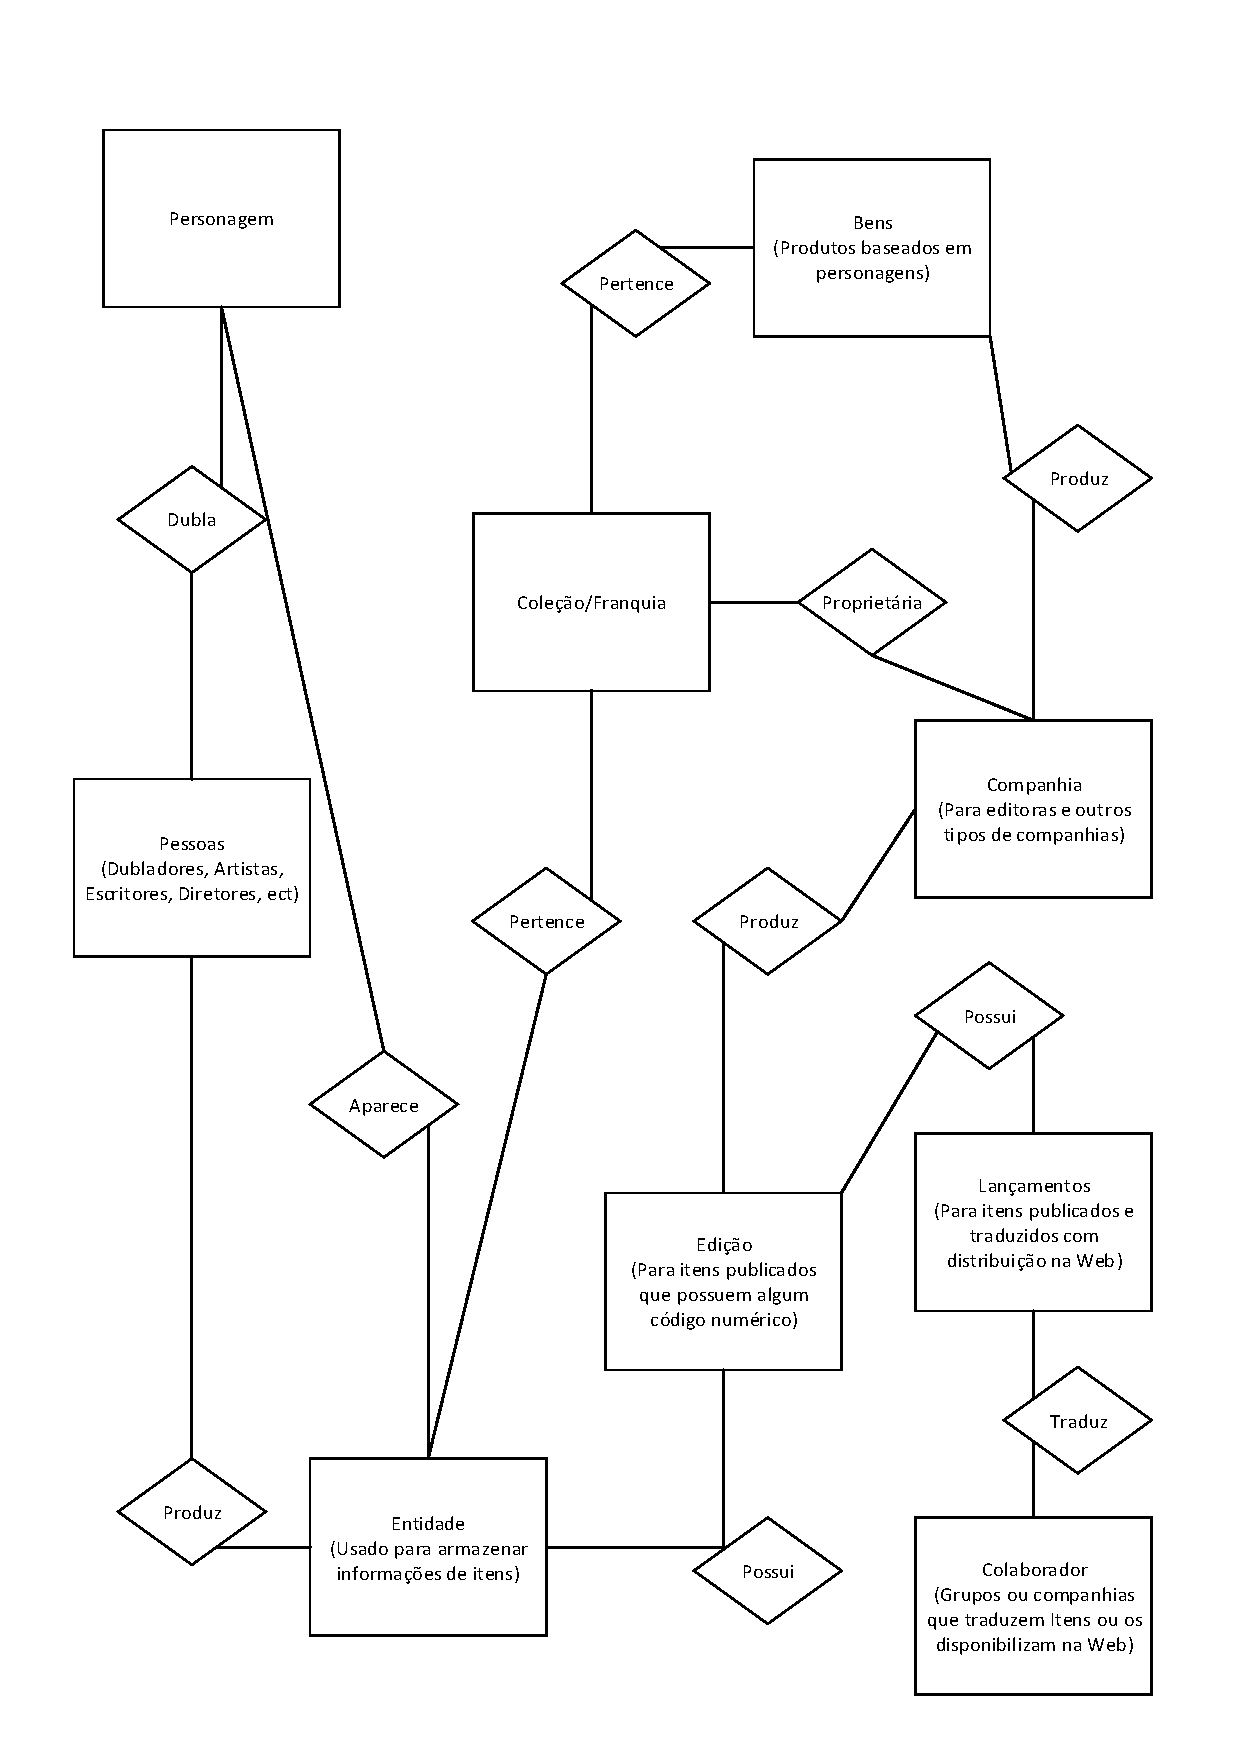
\includegraphics[width=1\textwidth]{MER_-_General.pdf}
\caption{Modelo Conceitual resumido com os nomes das principais entidades em português. No Modelo Conceitual detalhado e na implementação do Modelo Lógico foram utilizados textos em inglês.} \label{collection}
\end{figure}

A seguir podem ser observados as entidades e seus relacionamentos de forma mais detalhada. As entidades na cor laranja representam entidades que serão detalhadas mais a frente.
\begin{figure}[H]
\centering
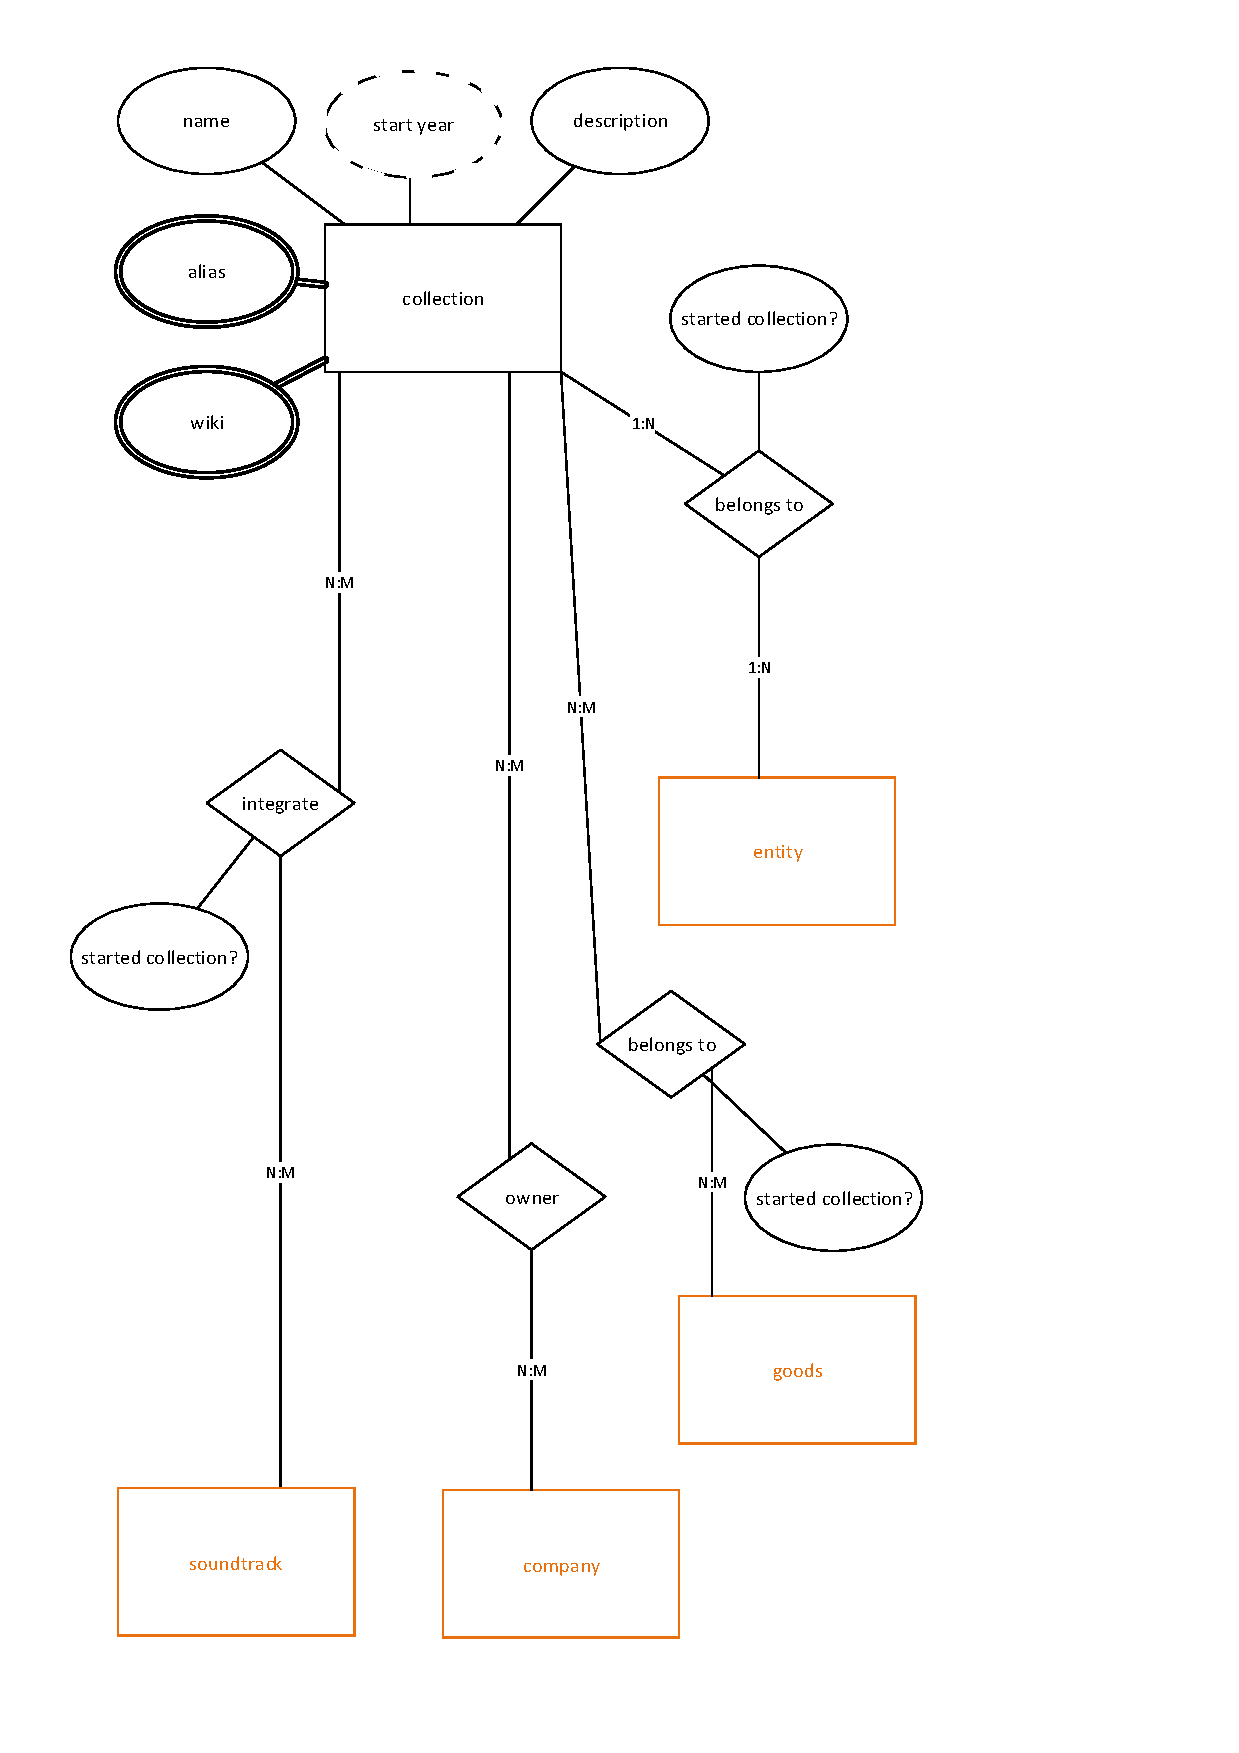
\includegraphics[height=0.85\textheight, width=0.75\textwidth]{MER_-_Collection.pdf}
\caption{\textit{Collection} é a entidade responsável por armazenar informações de franquias.} \label{collection}
\end{figure}

\begin{figure}[H]
\centering
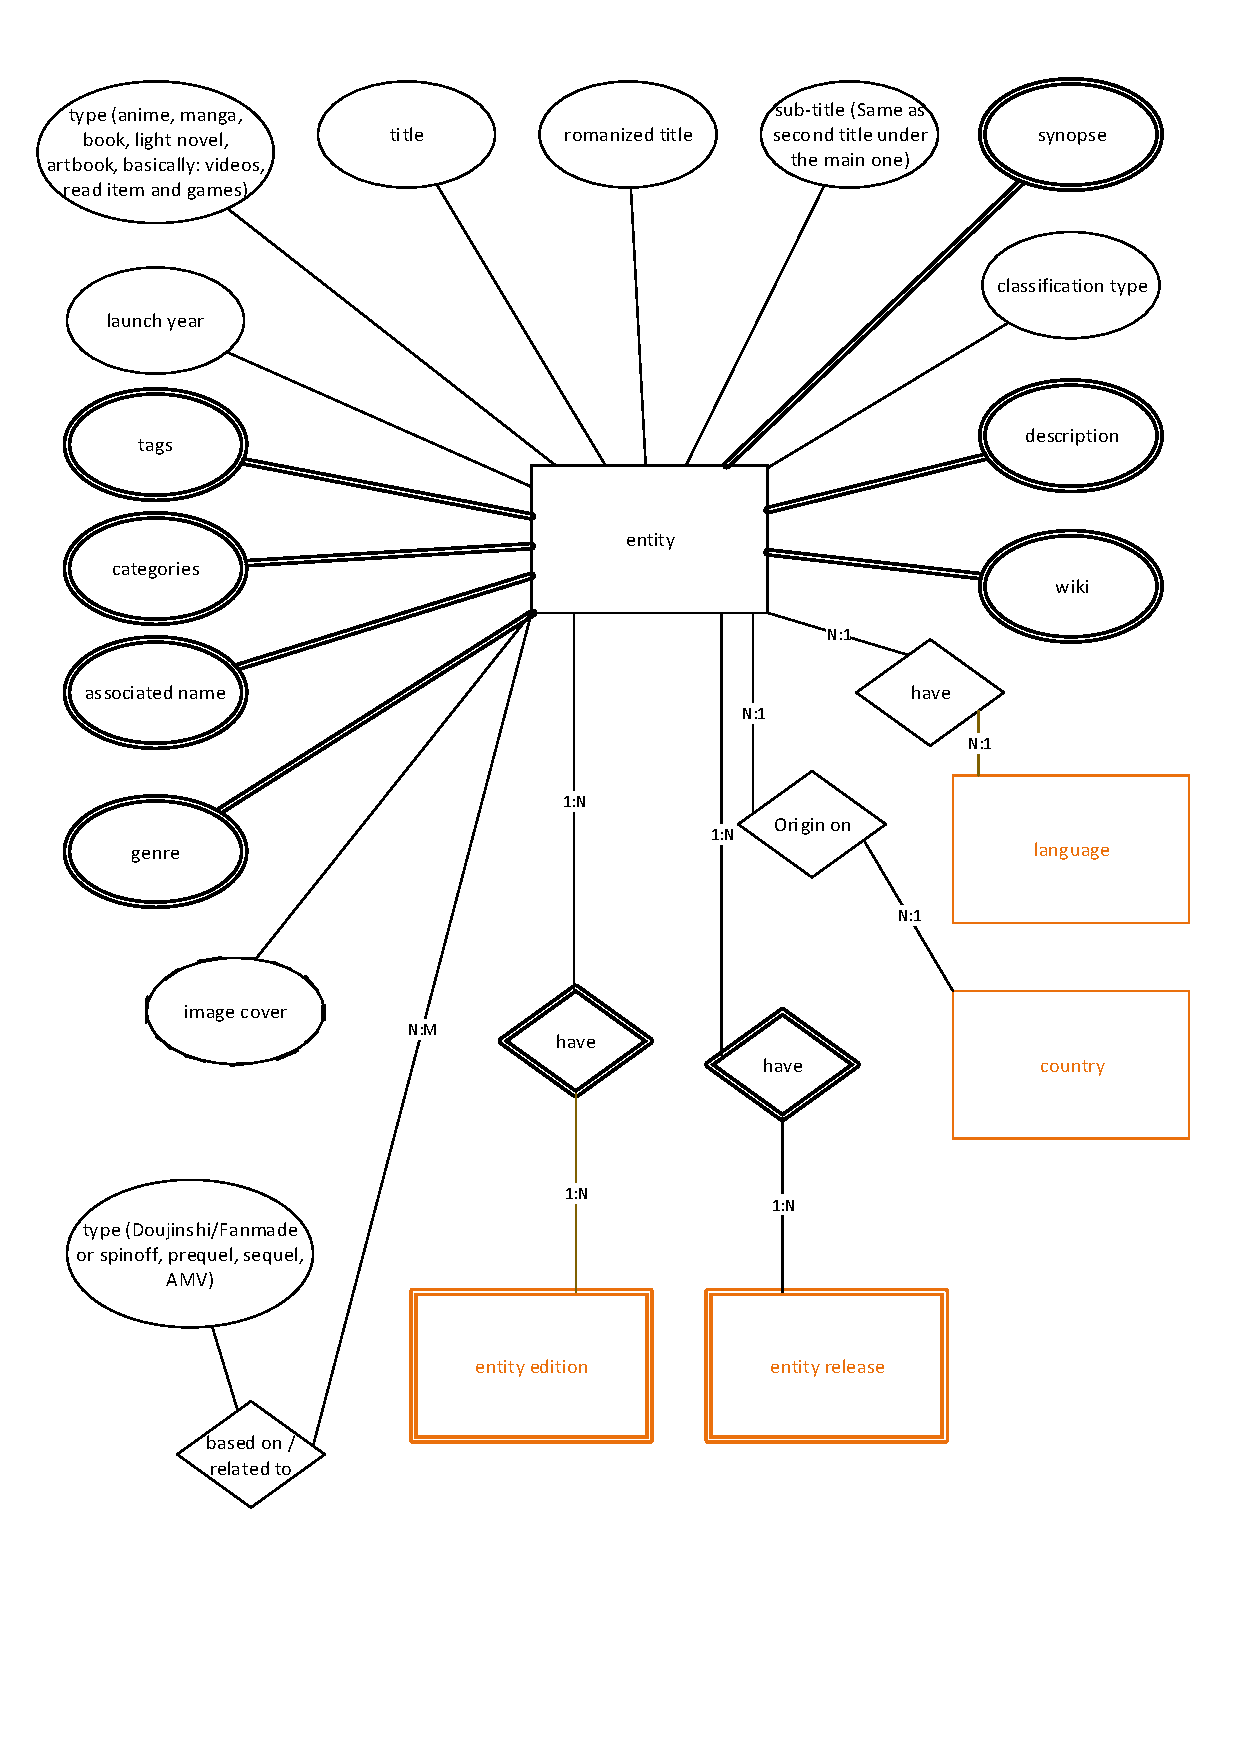
\includegraphics[width=1\textwidth]{MER_-_Entity.pdf}
\caption{\textit{Entity} é a entidade responsável por armazenar diversos tipos de conteúdo como vídeos, livros e jogos.} \label{entity}
\end{figure}

\begin{figure}[H]
\centering
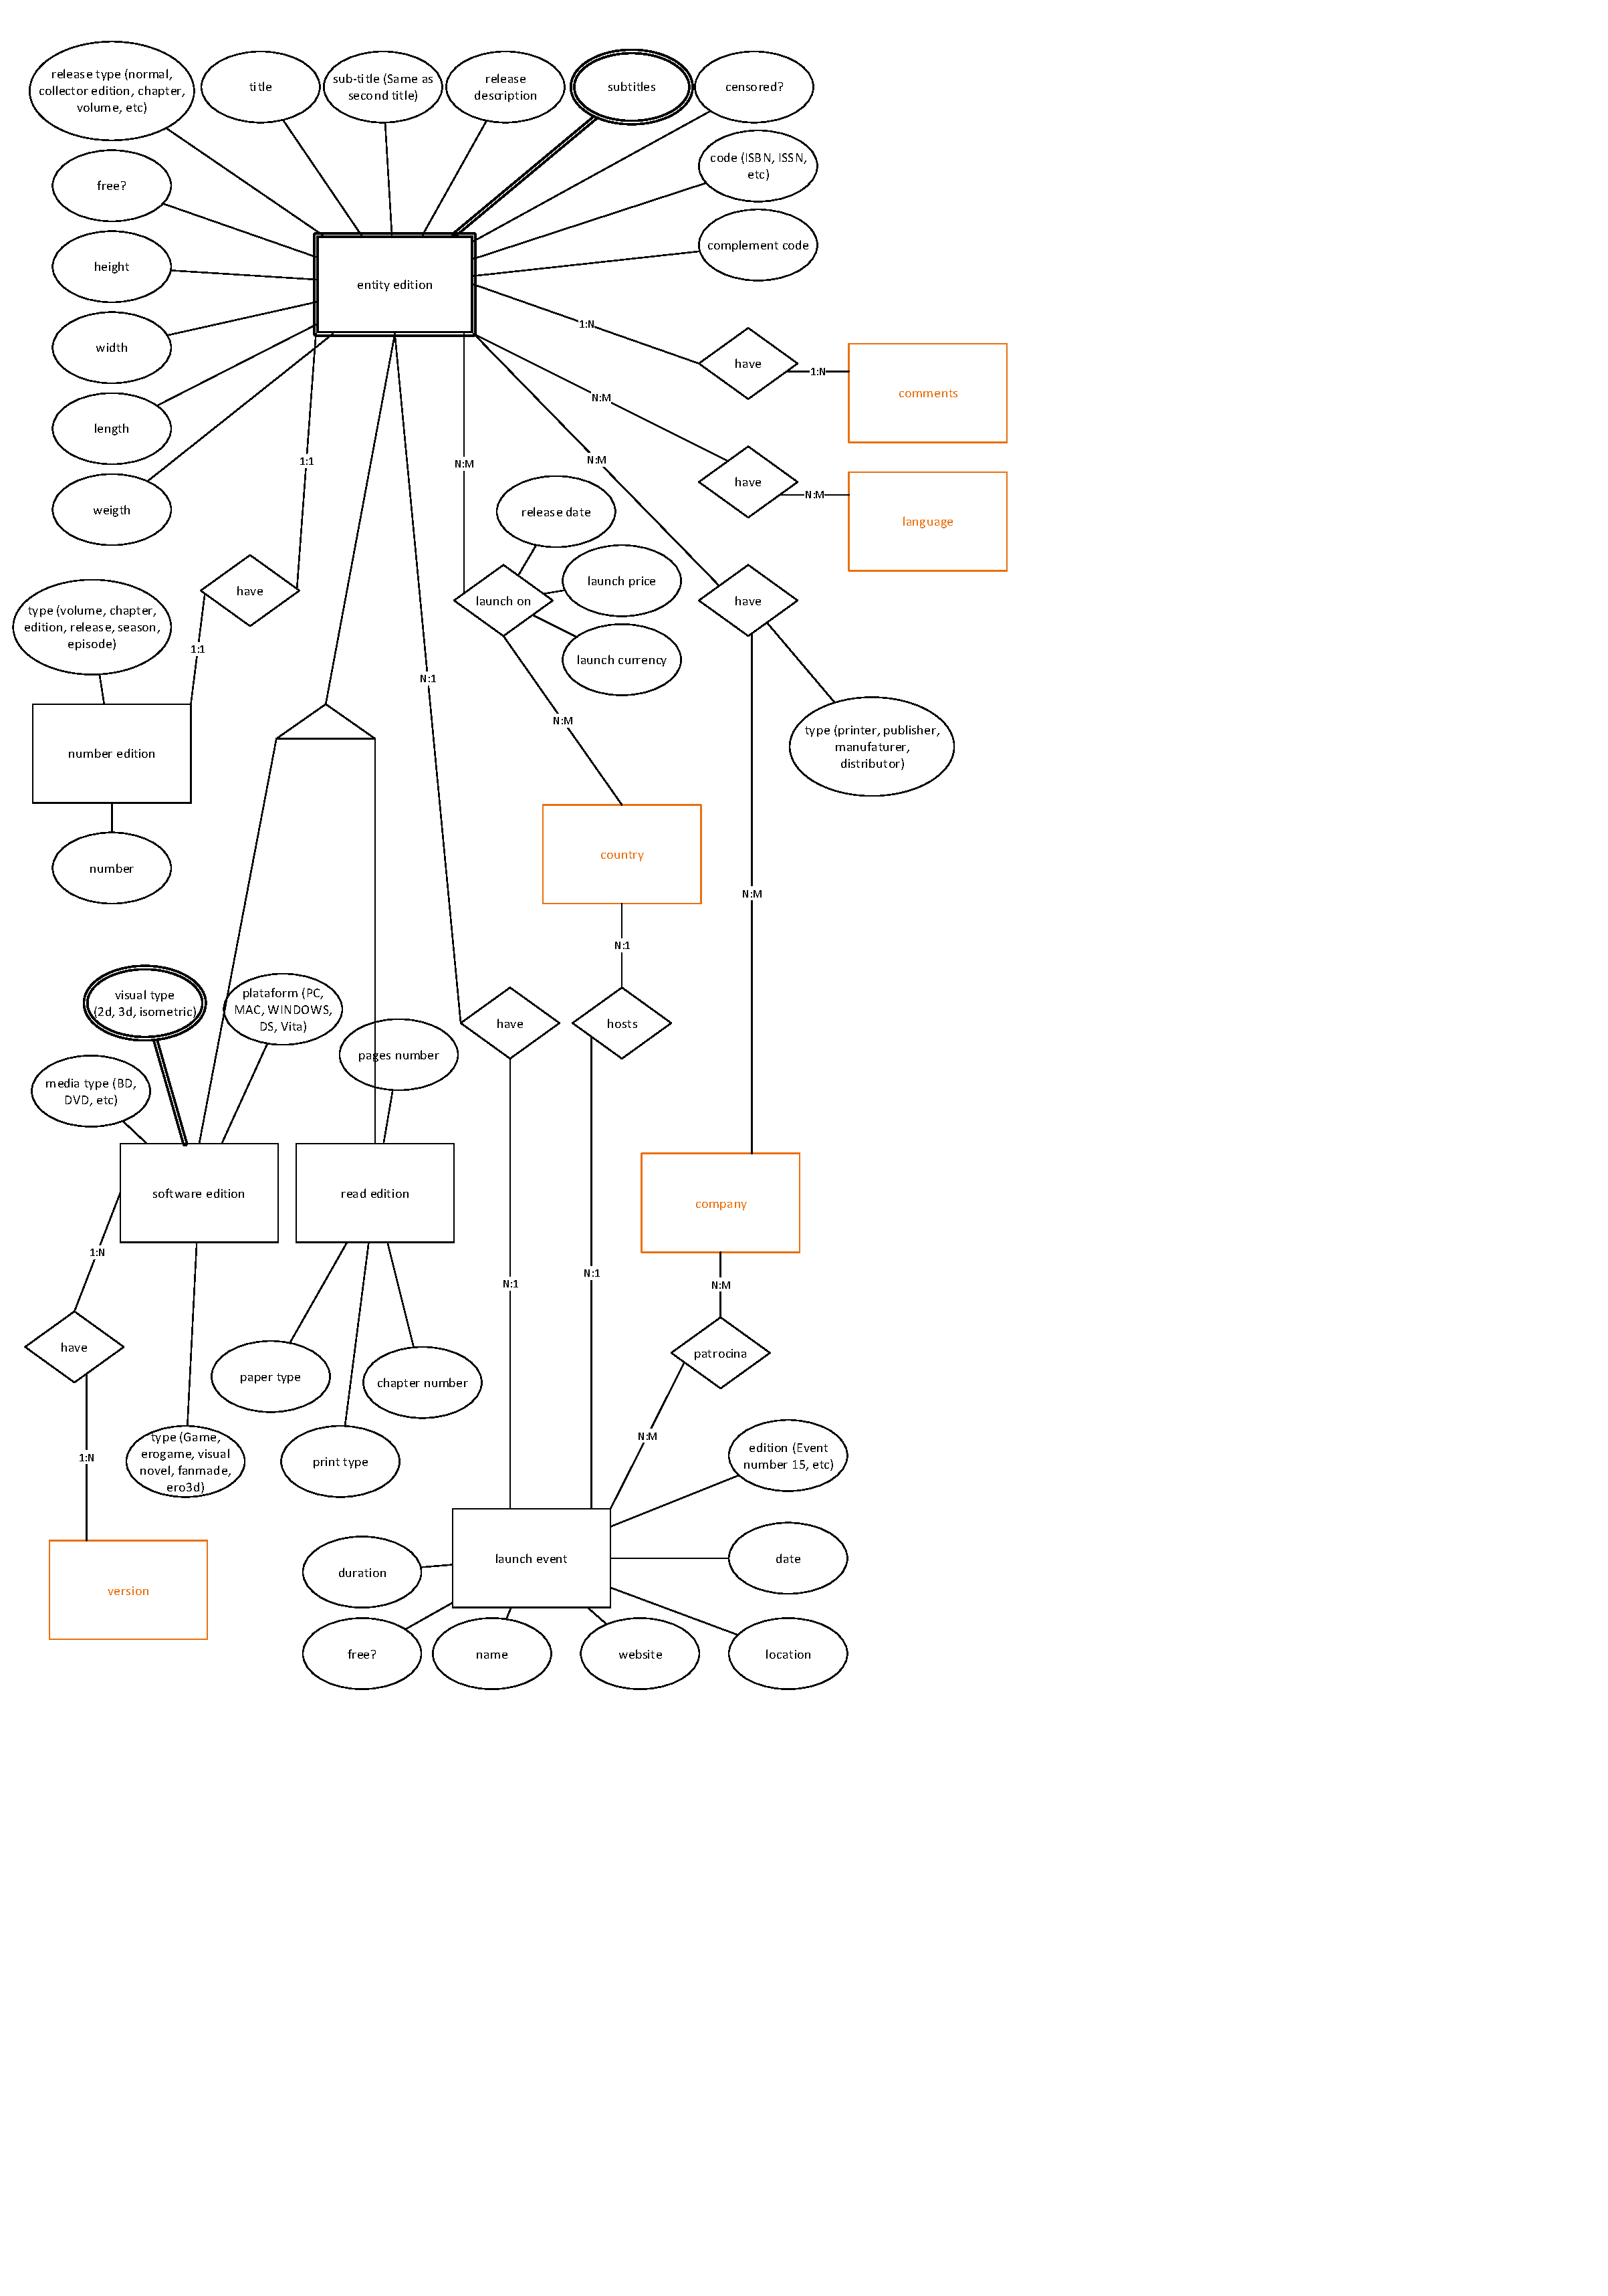
\includegraphics[height=0.9\textheight,width=0.9\textwidth]{MER_-_Edition.pdf}
\caption{\textit{Edition} é a entidade responsável por armazenar informações de itens armazenados em \textit{Entity} que possuem publicação física. A entidade \textit{Edition} se especializa em \textit{Software Edition} para armazenamento de informações especificas a softwares e \textit{Read Edition} para armazenamento de informações de livros e revistas}\label{edition}
\end{figure}

\begin{figure}[H]
\centering
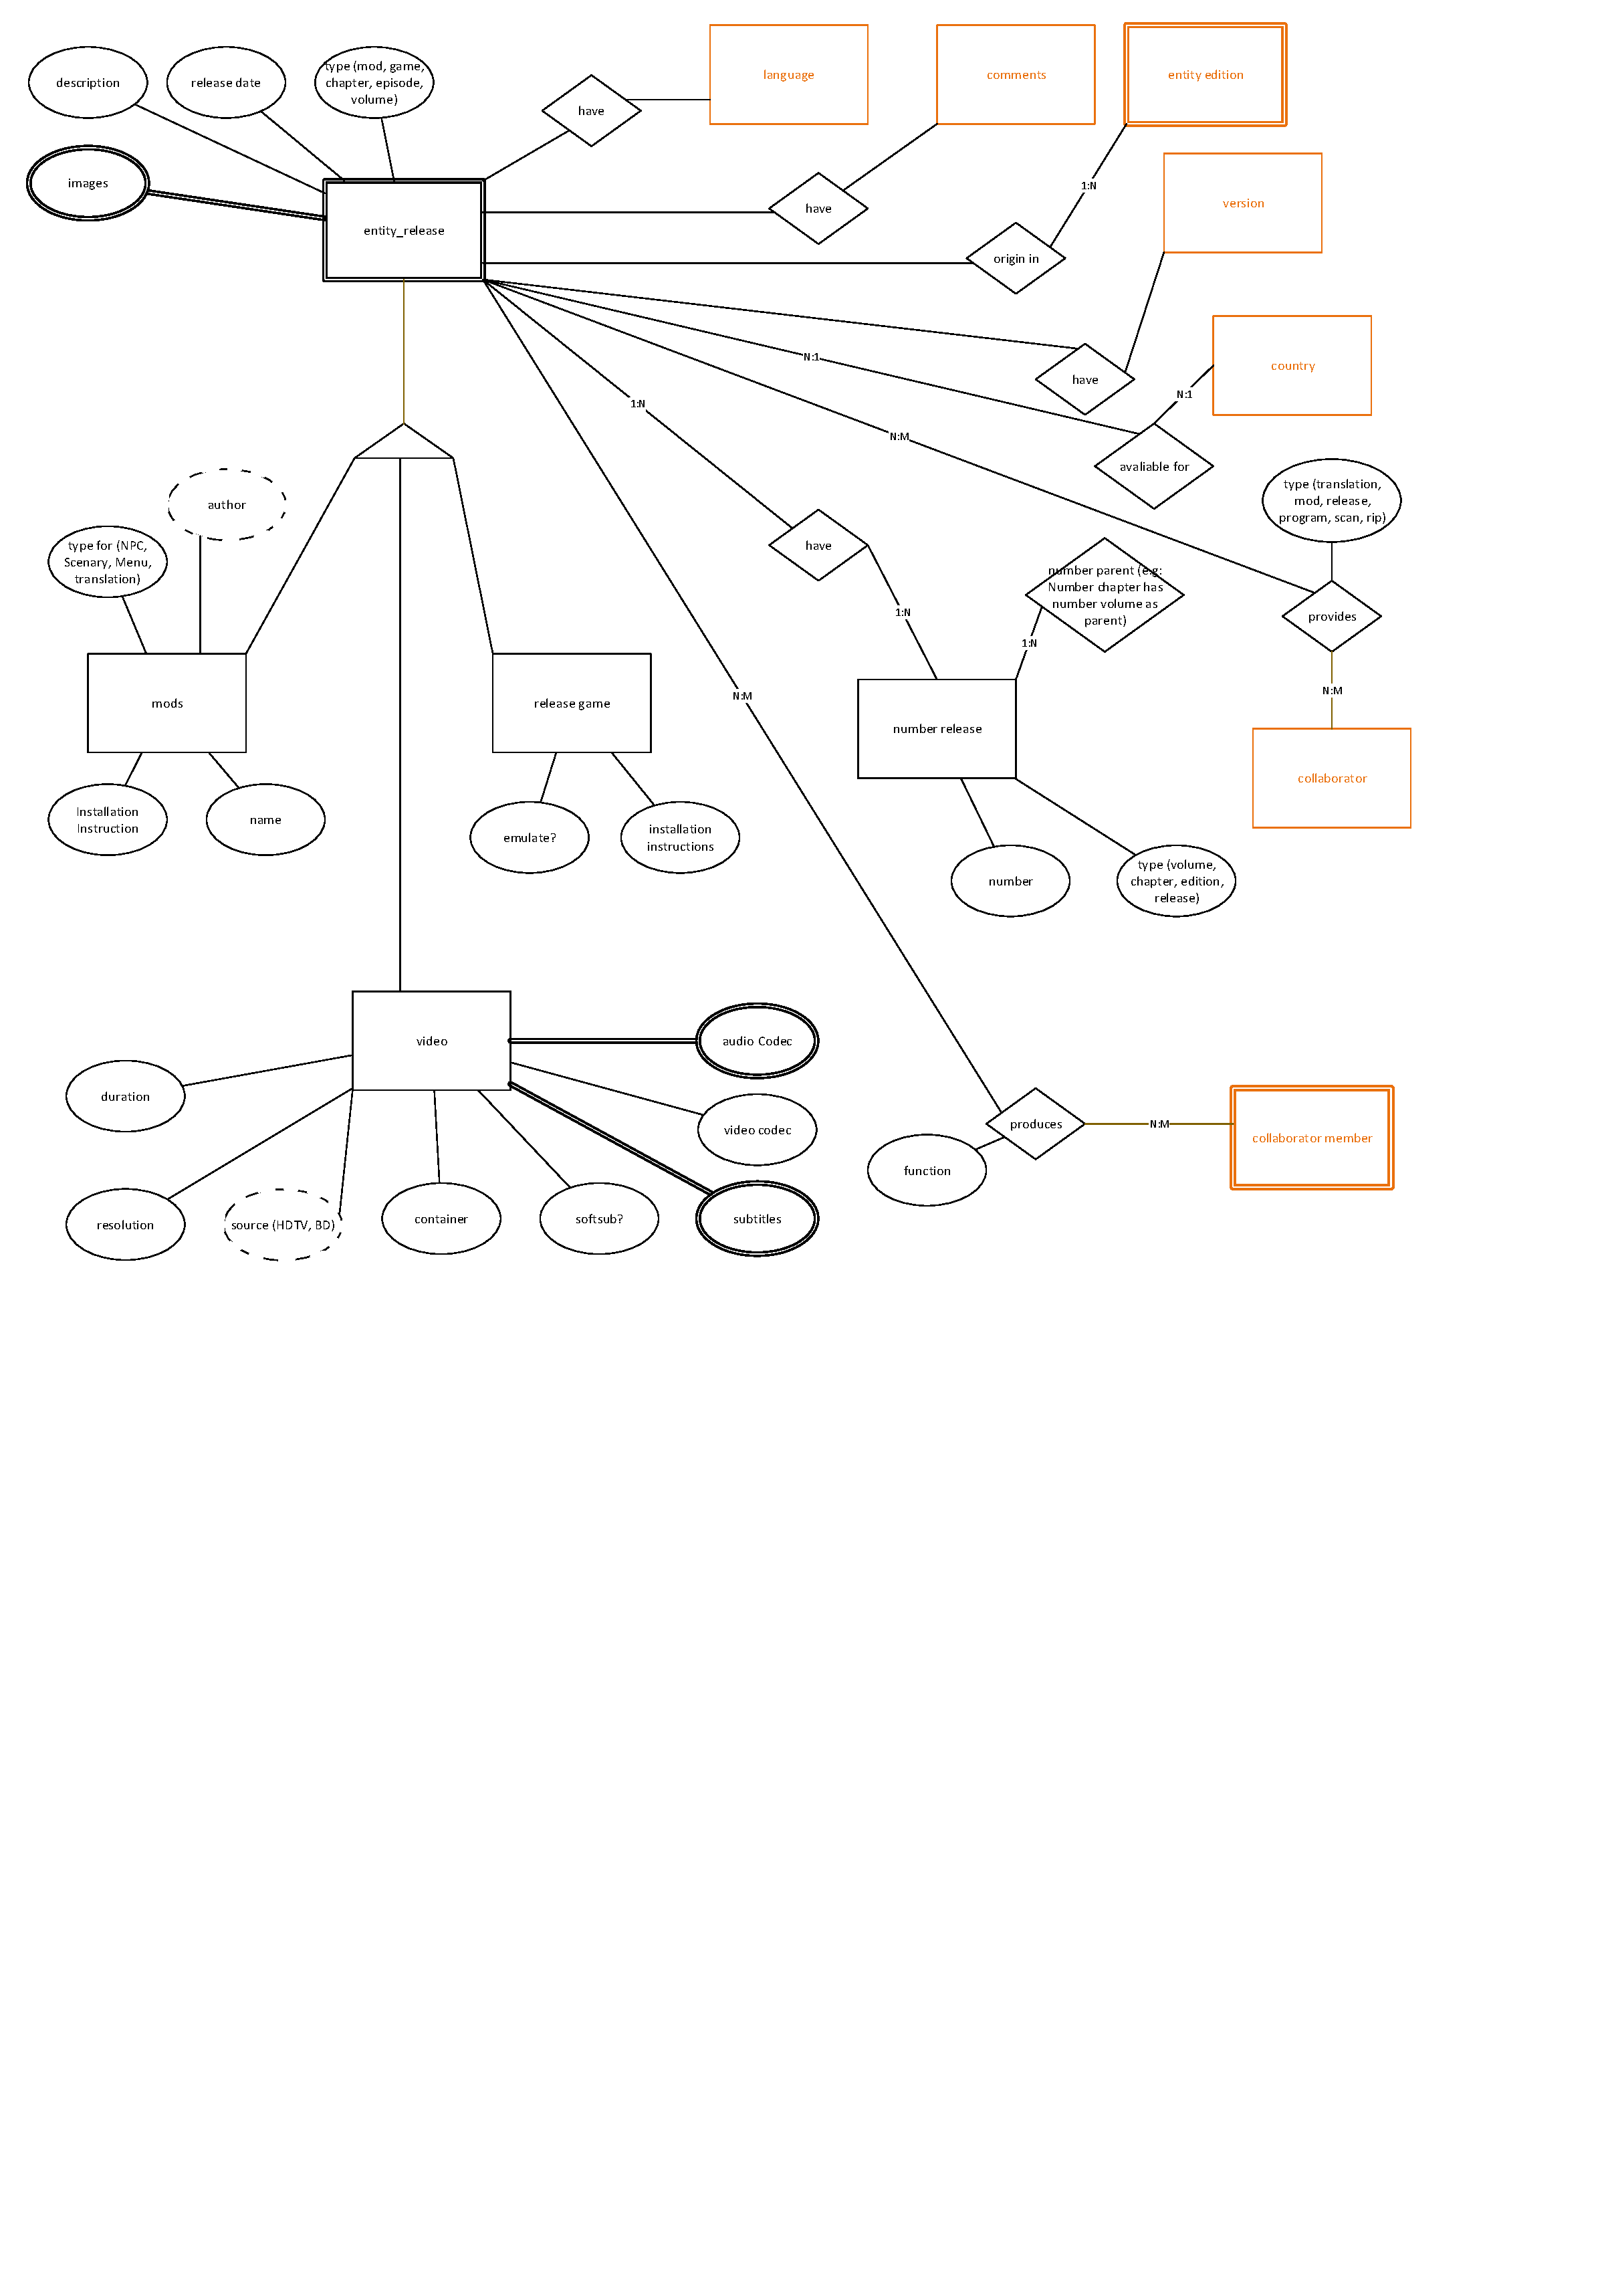
\includegraphics[height=0.8\textheight,width=1.1\textwidth]{MER_-_Release.pdf}
\caption{Entidades responsáveis pelo armazenamento de conteúdo disponibilizado na web como modificações de jogos, conhecidos pela abreviação Mod, de traduções não oficiais de conteúdo ainda não licenciado fora do Japão e de distribuições de conteúdos, legalmente, através da Web.} \label{Release}
\end{figure}

\begin{figure}[H]
\centering
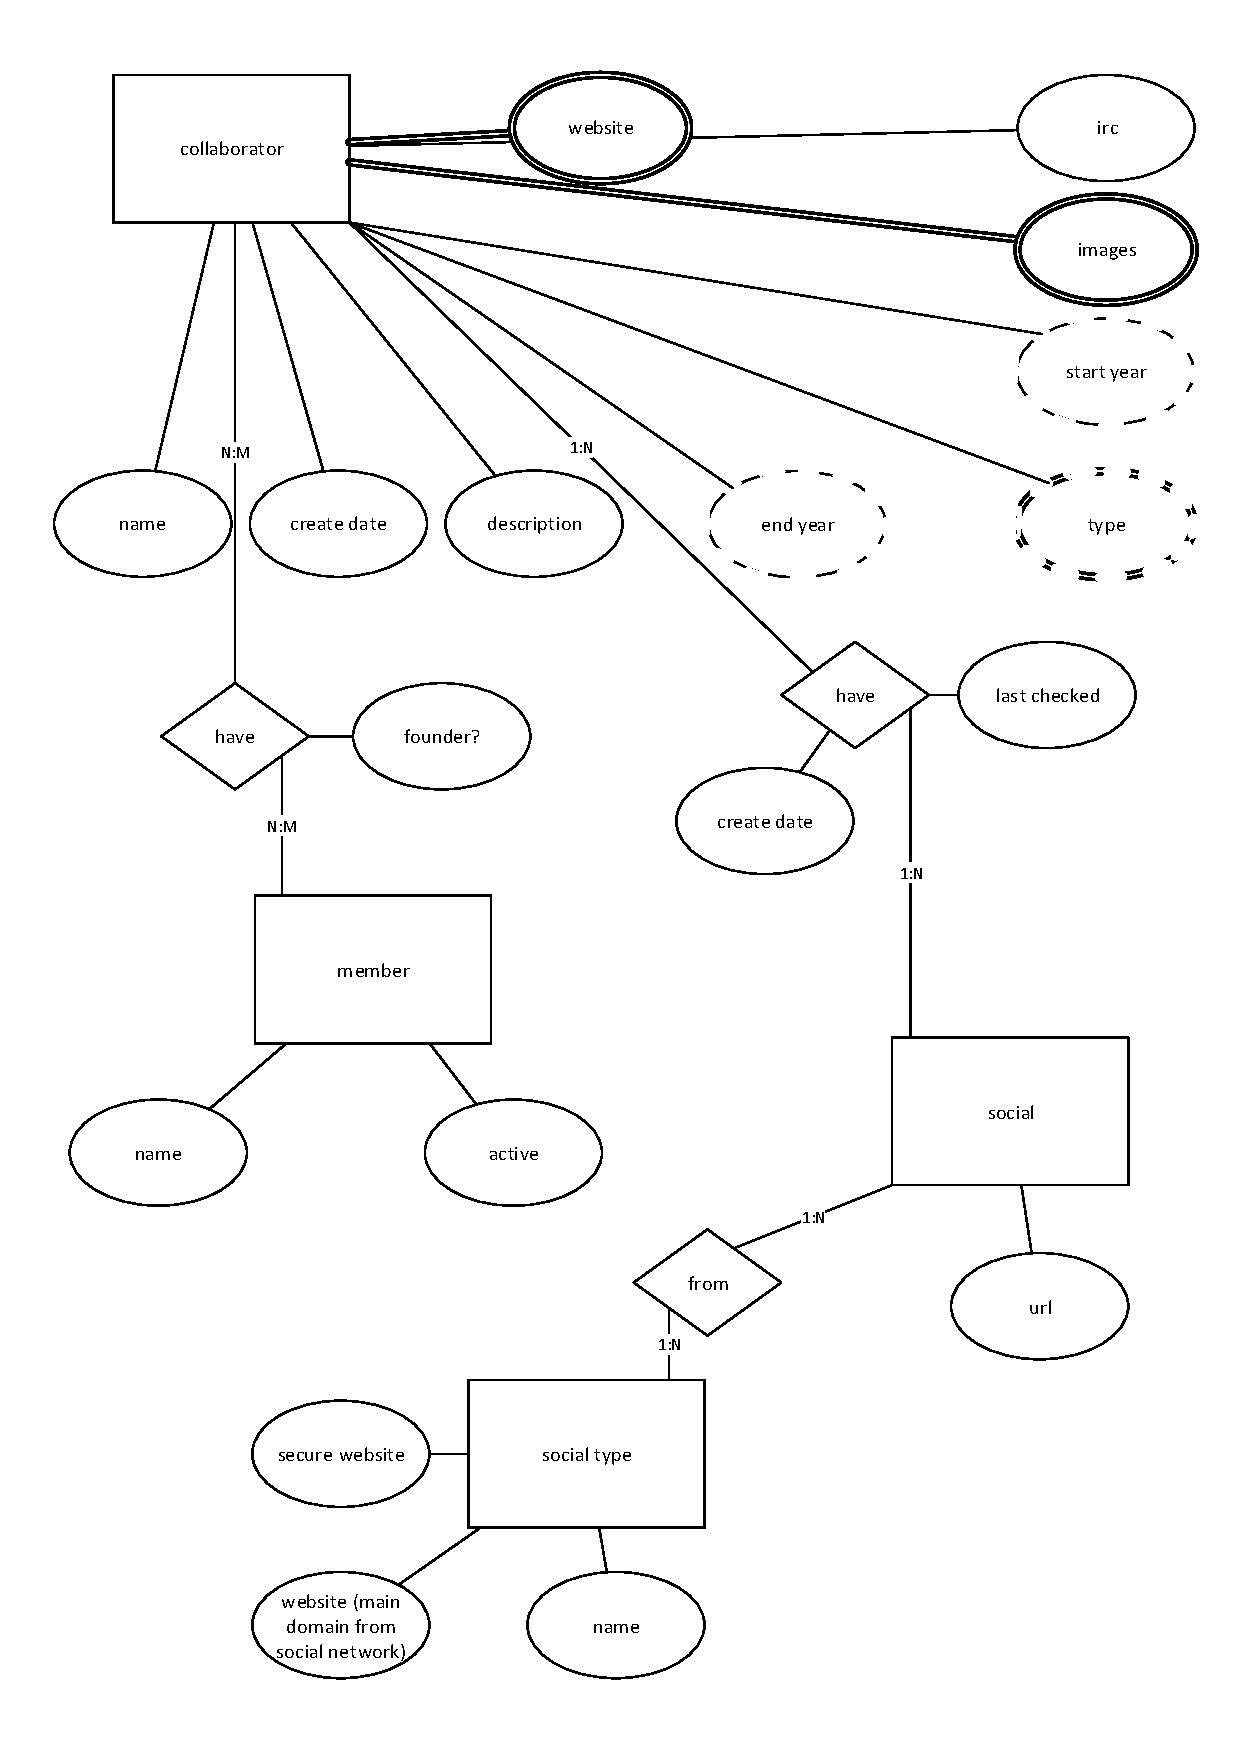
\includegraphics[width=1\textwidth]{MER_-_Collaborator_Social.pdf}
\caption{Entidades com informações sobre grupos de tradução ou distribuidores de conteúdo digital, seus membros e suas redes sociais.} \label{collaborator}
\end{figure}


\begin{figure}[H]
\centering
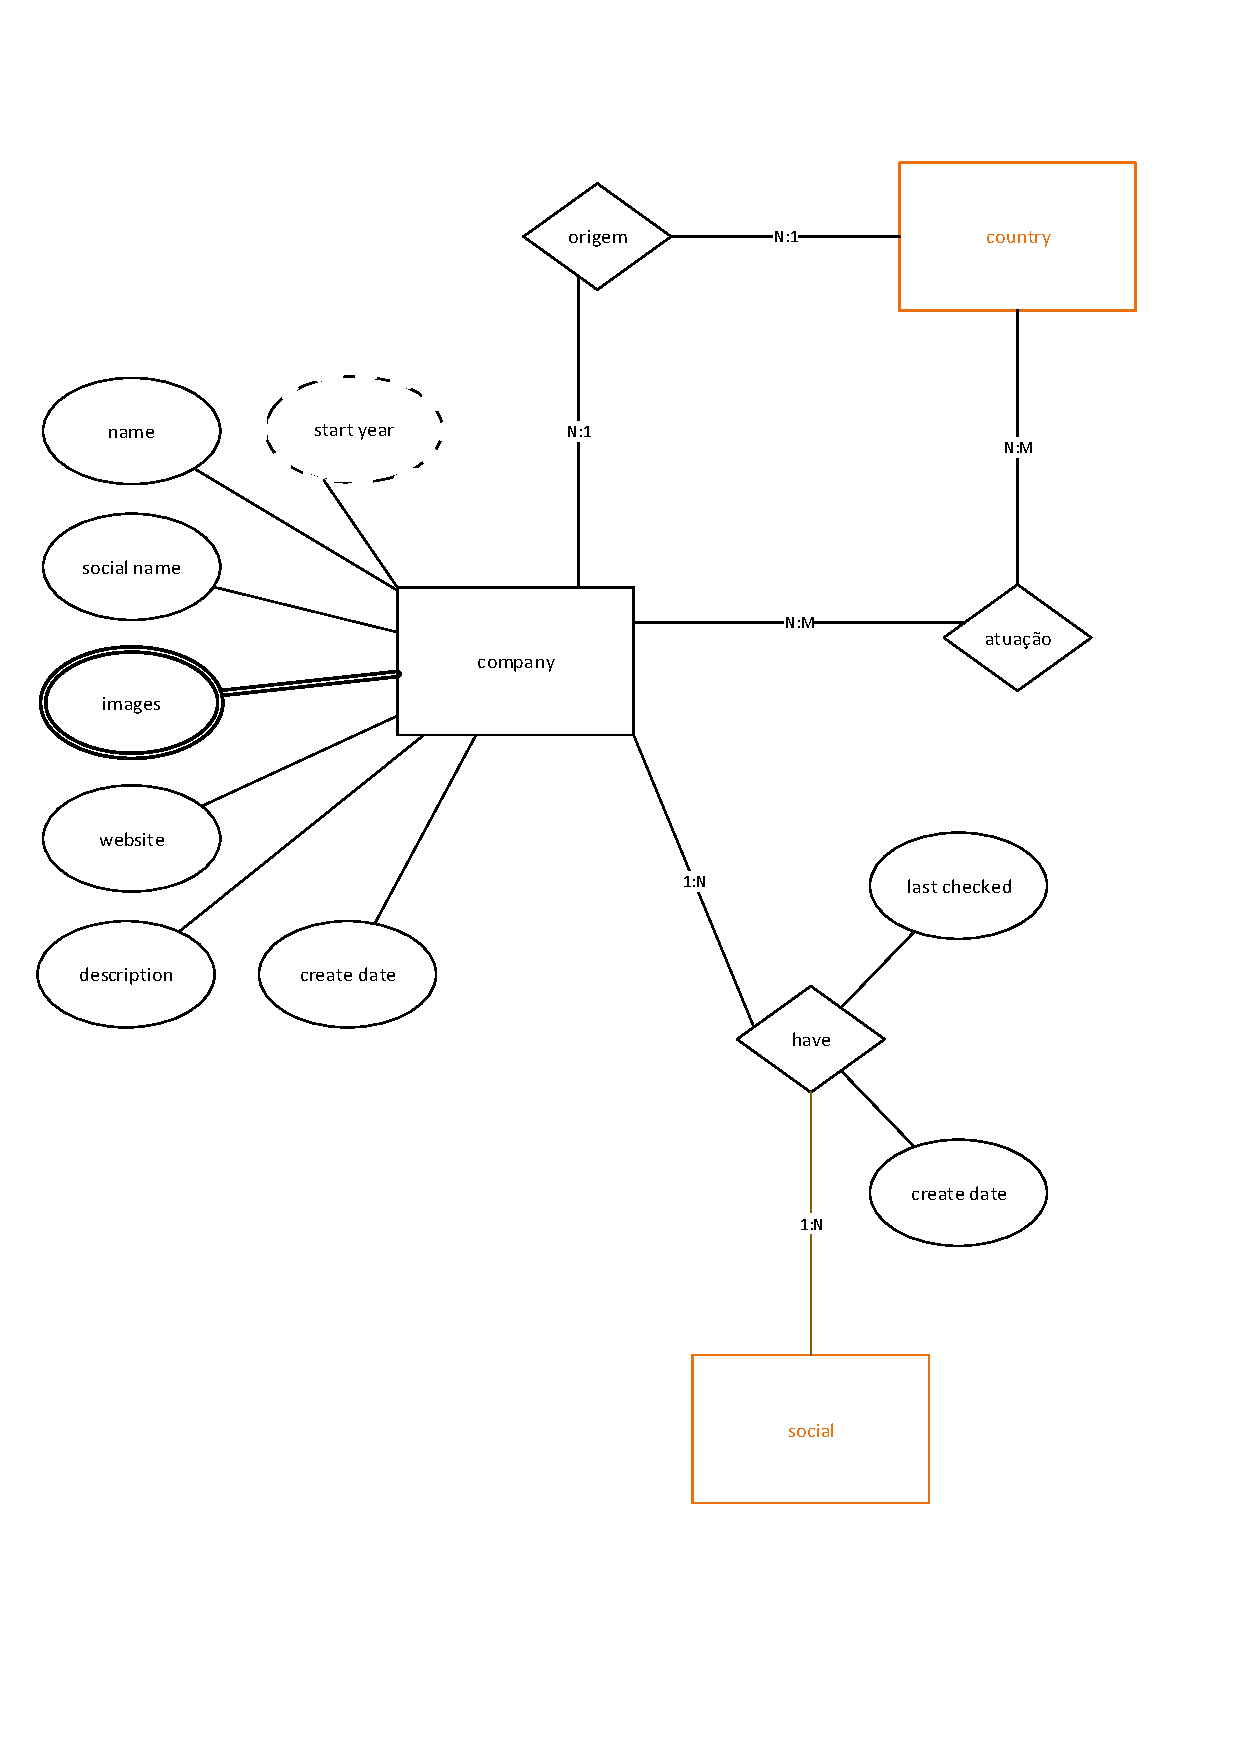
\includegraphics[width=1\textwidth]{MER_-_Company.pdf}
\caption{\textit{Company} é a entidade responsável por armazenar informações de diversas empresas envolvidas na produção de itens. Atributo \textit{images} é utilizado para armazenar apenas a referência das imagens, uma vez que imagens não são armazenadas diretamente no banco de dados.}\label{company}
\end{figure}

\begin{figure}[H]
\centering
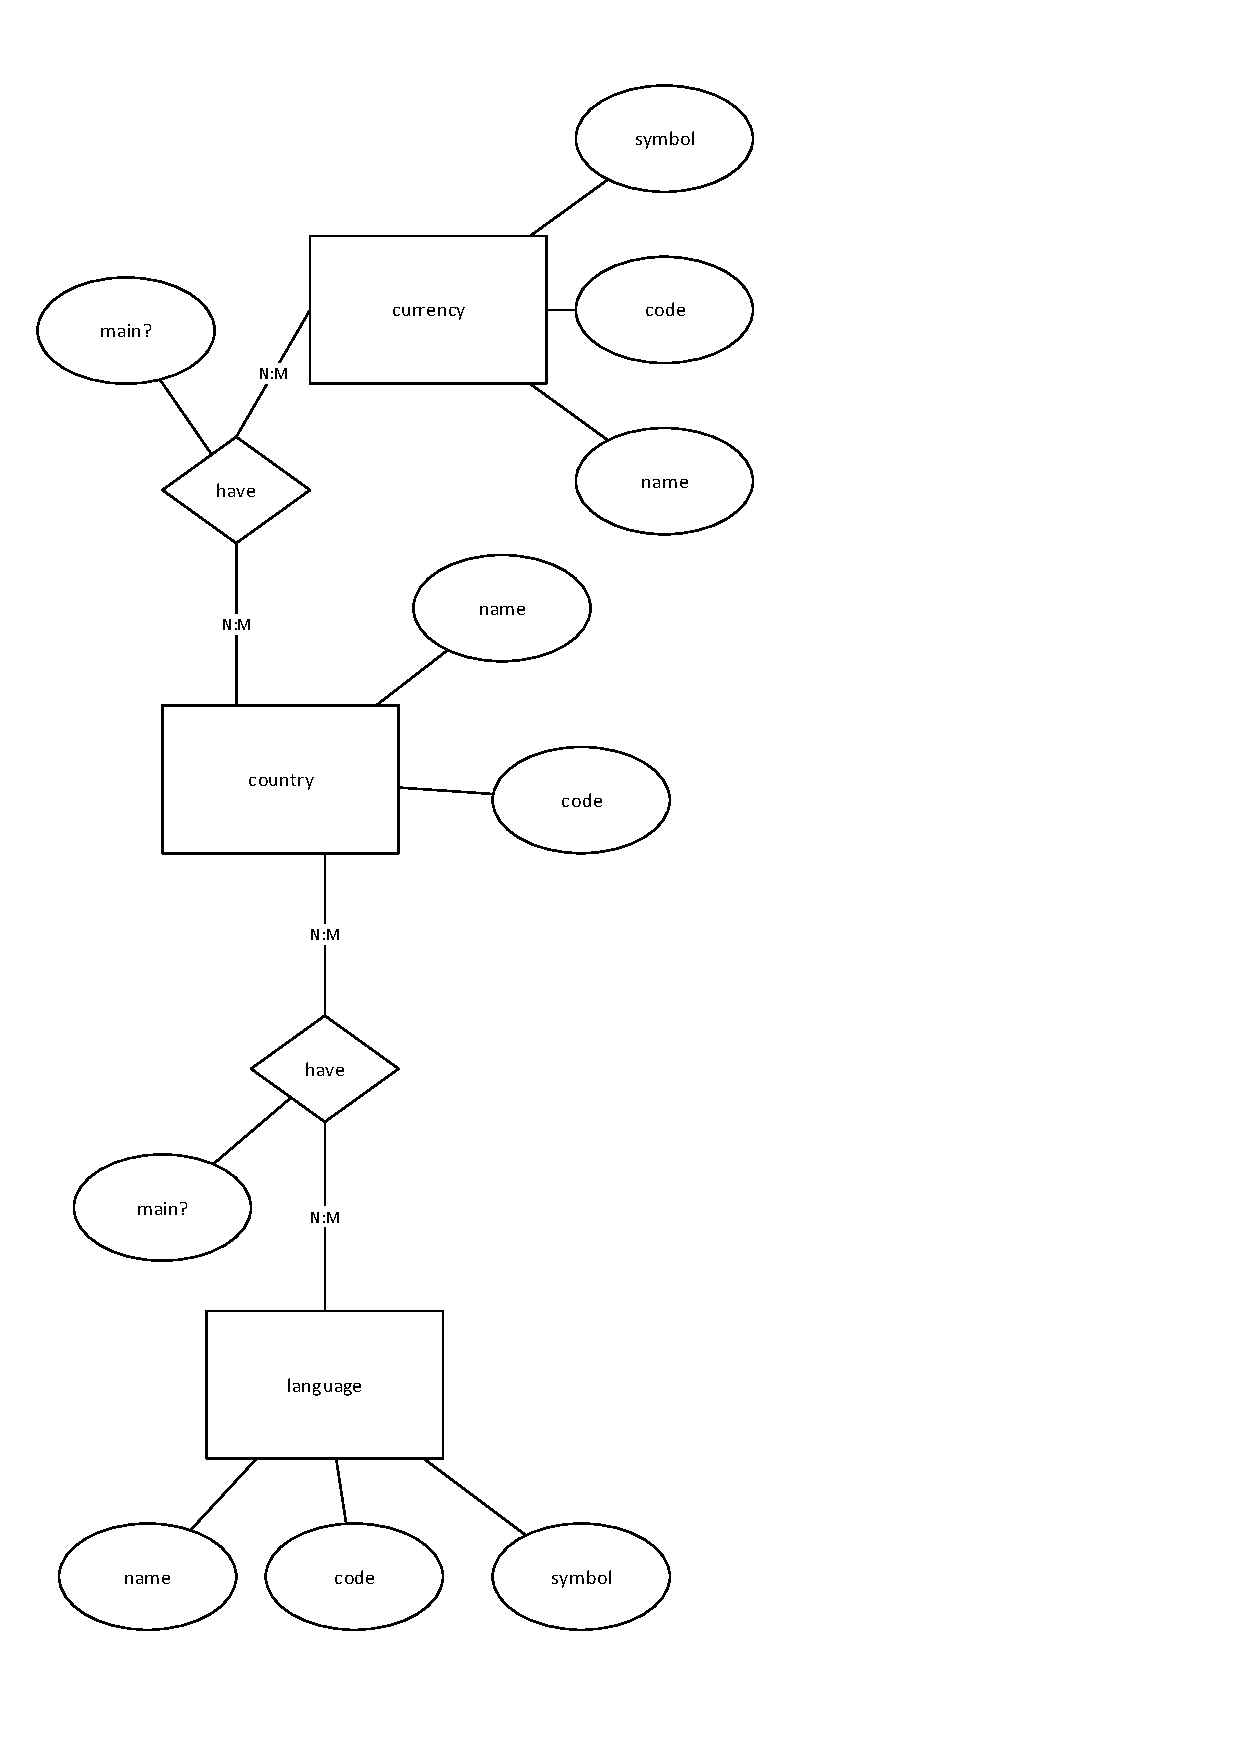
\includegraphics[height=0.92\textheight,width=0.70\textwidth]{MER_-_Country-Language-Currency.pdf}
\caption{Entidades responsáveis pelo armazenamento de informações de países, seus idiomas e suas moedas.} \label{hash}
\end{figure}

\begin{figure}[H]
\centering
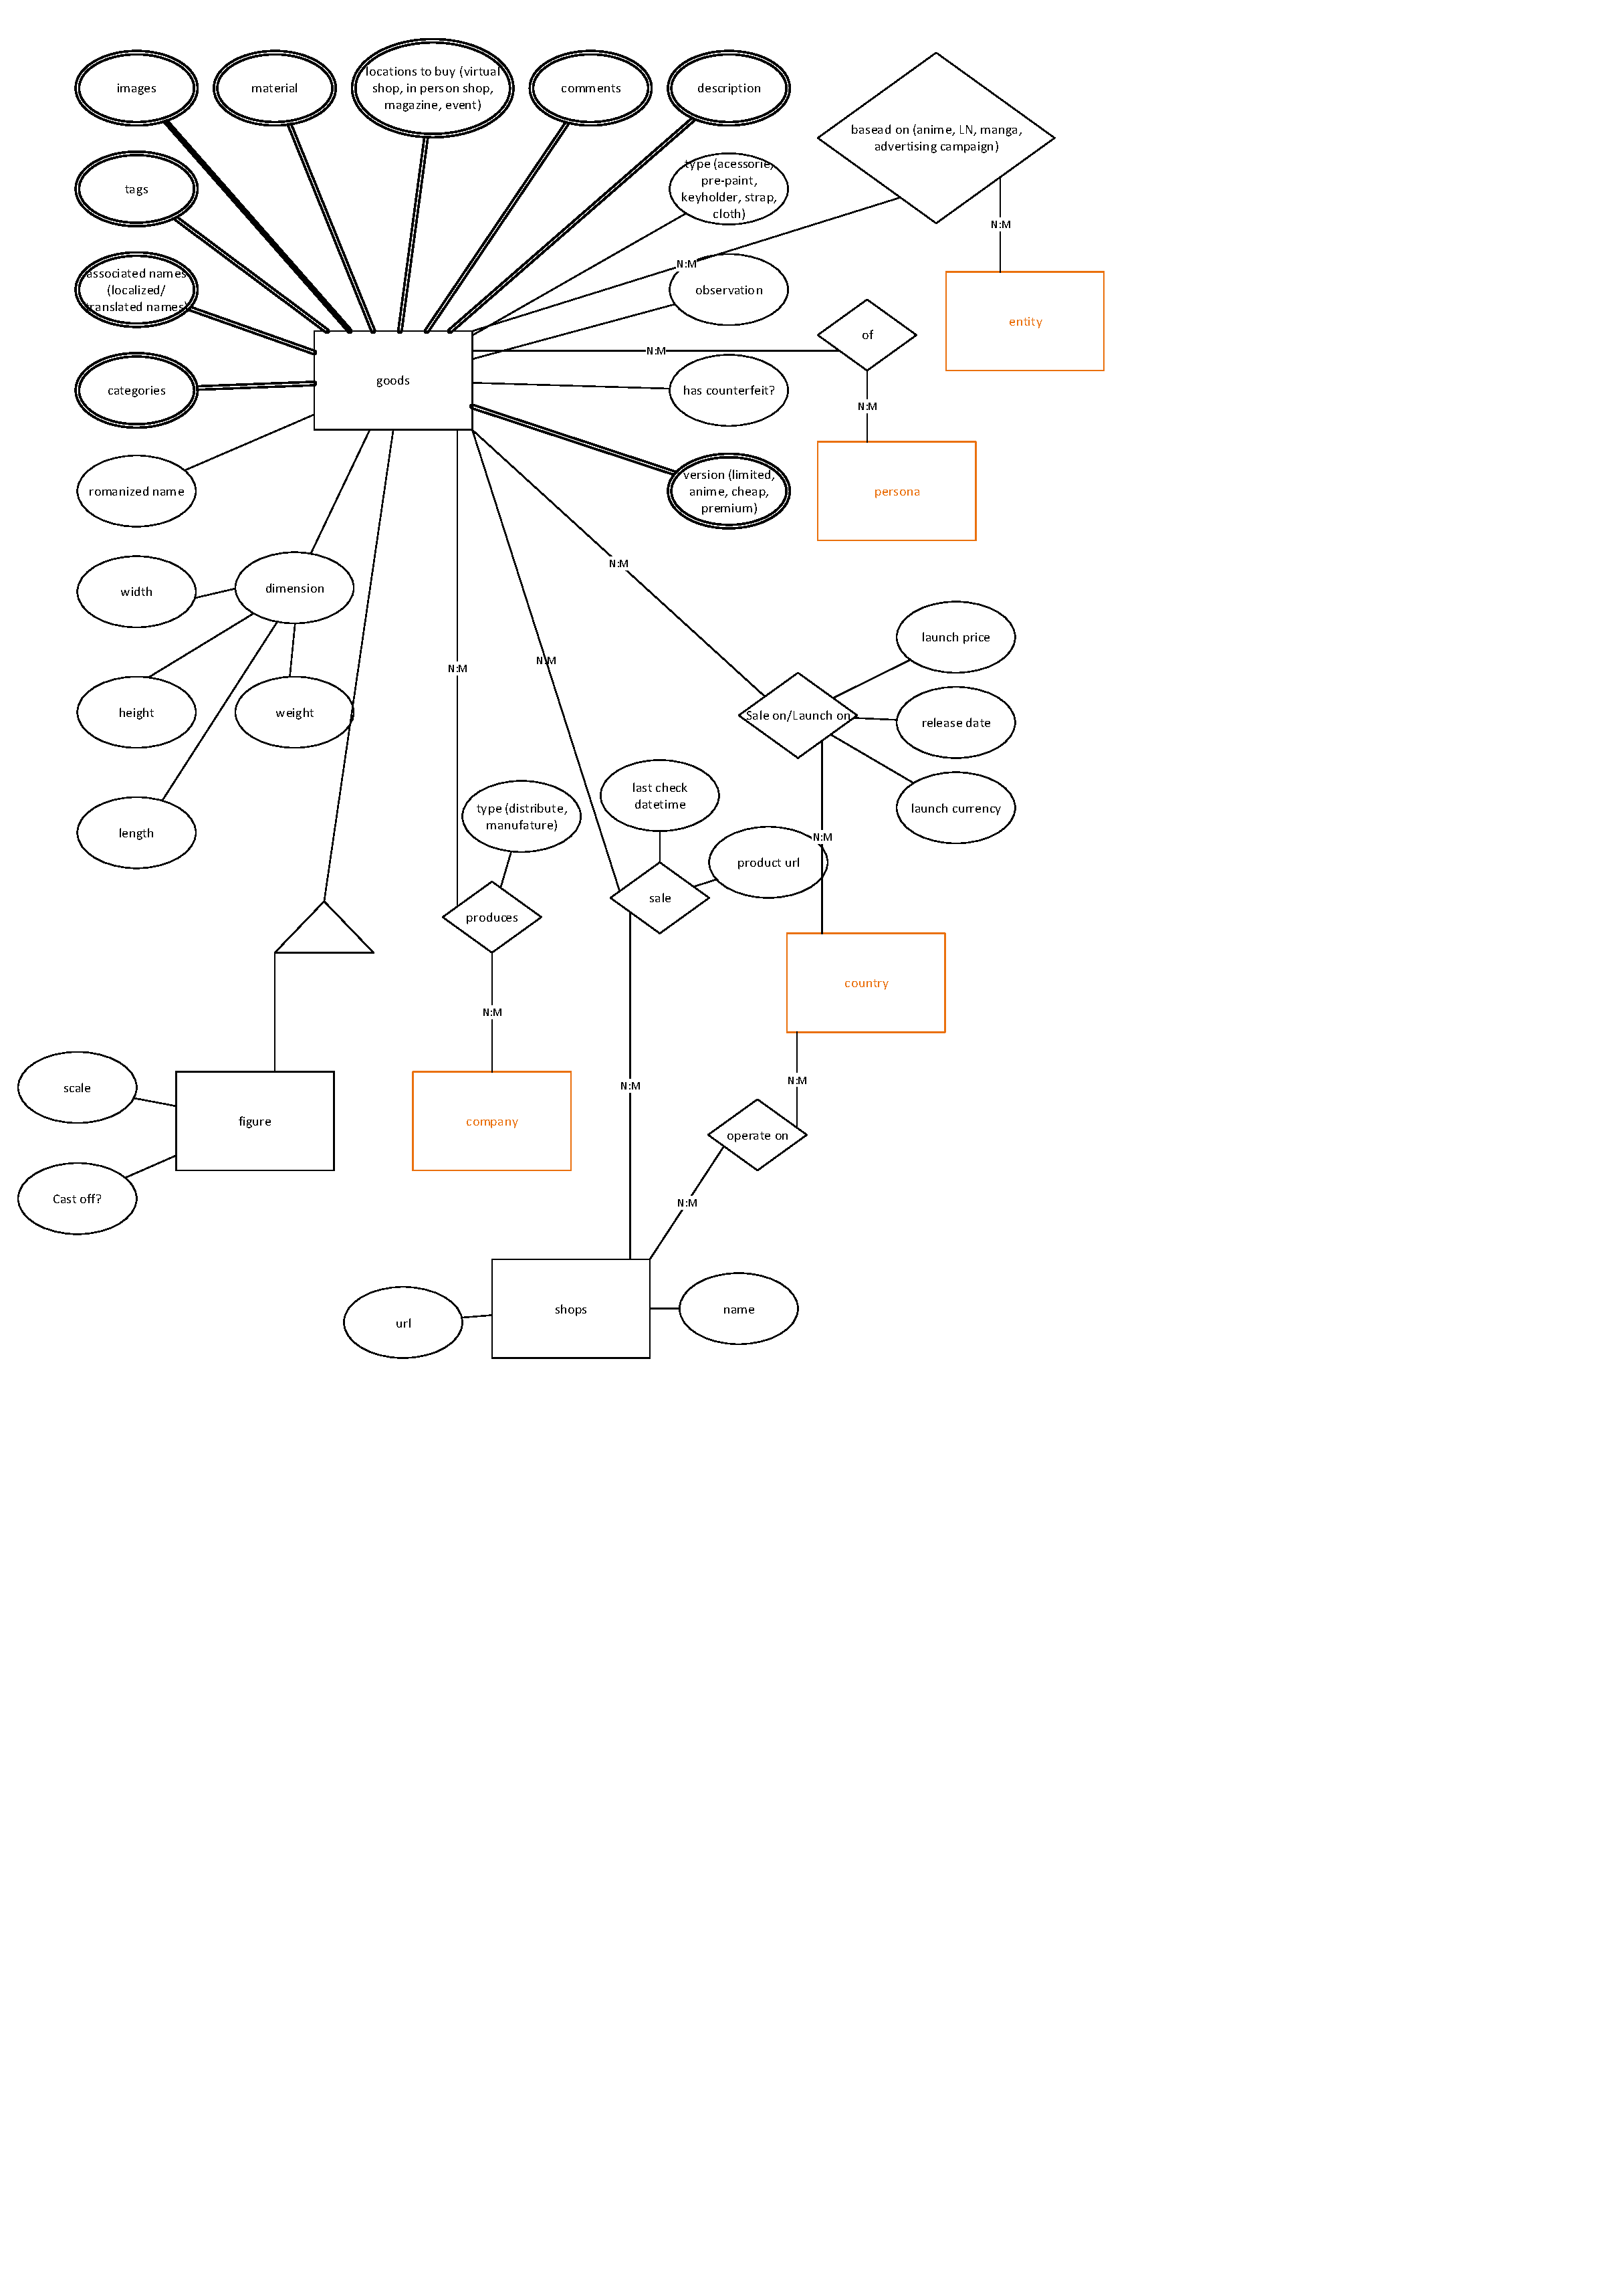
\includegraphics[height=0.98\textheight,width=1.1\textwidth]{MER_-_Goods.pdf}
\caption{Entidade \textit{Goods} se especializa em \textit{Figure}.} \label{goods}
\end{figure}

\begin{figure}[H]
\centering
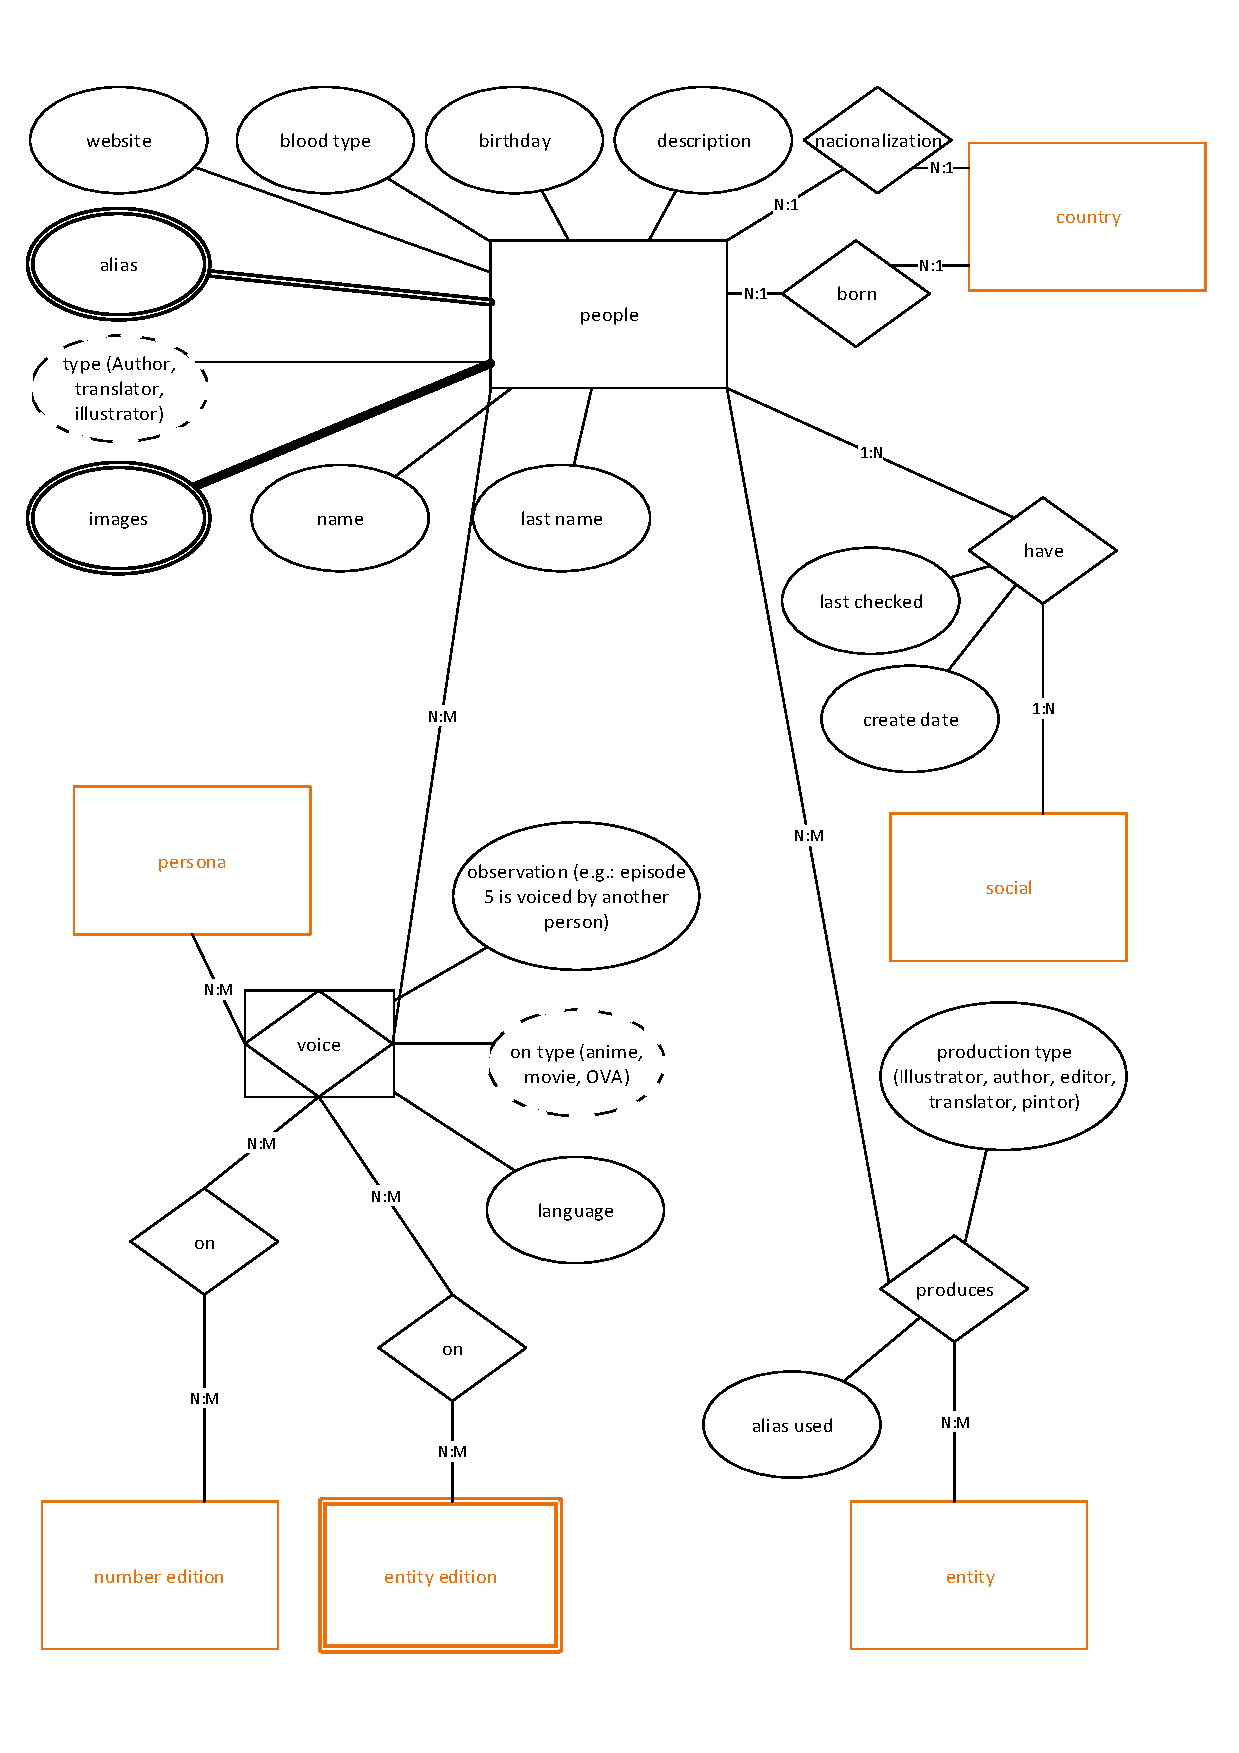
\includegraphics[height=0.92\textheight,width=1\textwidth]{MER_-_People.pdf}
\caption{Entidades responsáveis pelo armazenamento de informações de pessoas envolvidas na produção de itens. Entre o relacionamento de pessoas com personagens há associação utilizada para indicar em quais edições e episódios (\textit{number edition}) o dublador participou. Há situações onde o dublador oficial não pode dublar um episódio ou uma lista de episódios por motivos fora de seu controle.} \label{hash}
\end{figure}

\begin{figure}[H]
\centering
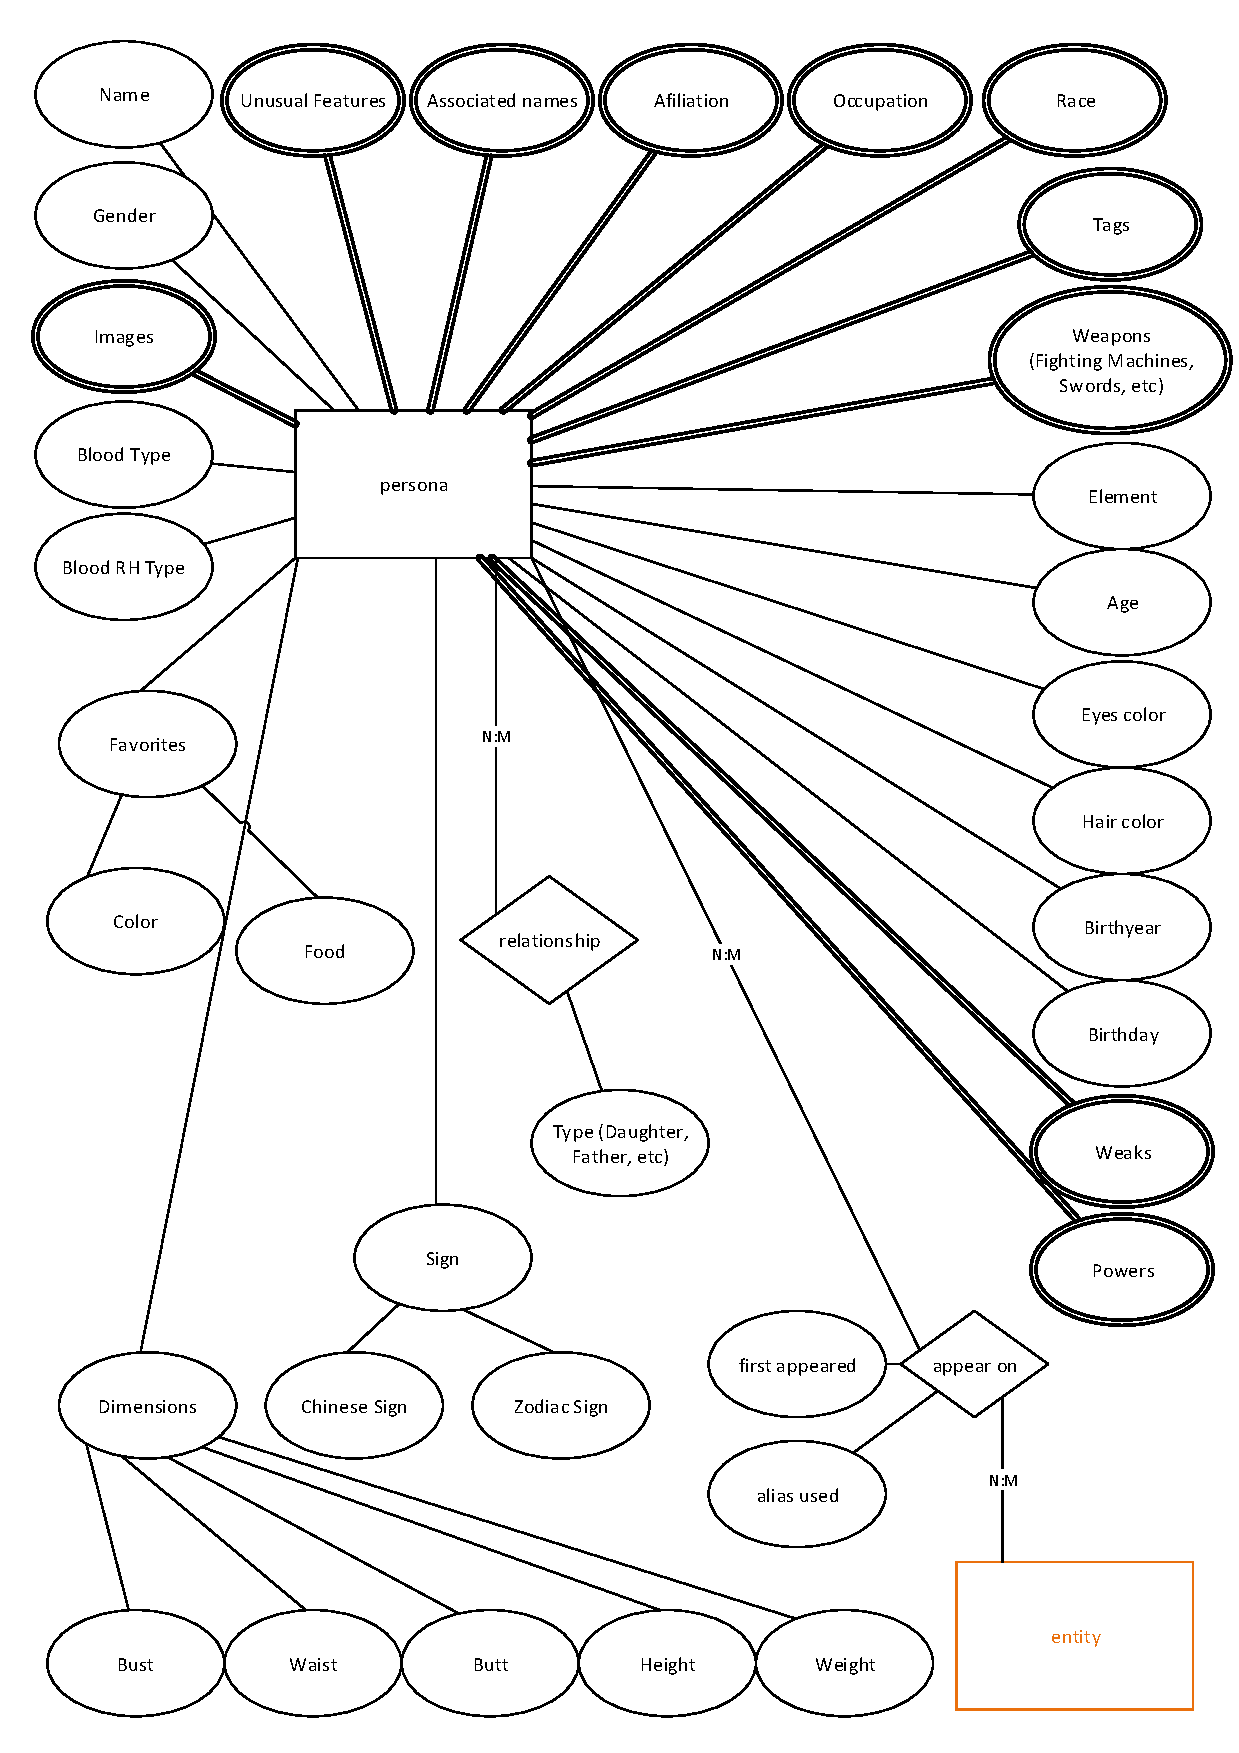
\includegraphics[width=1\textwidth]{MER_-_Persona.pdf}
\caption{Entidade responsável por armazenas personagens e suas características.} \label{Persona}
\end{figure}


\begin{figure}[H]
\centering
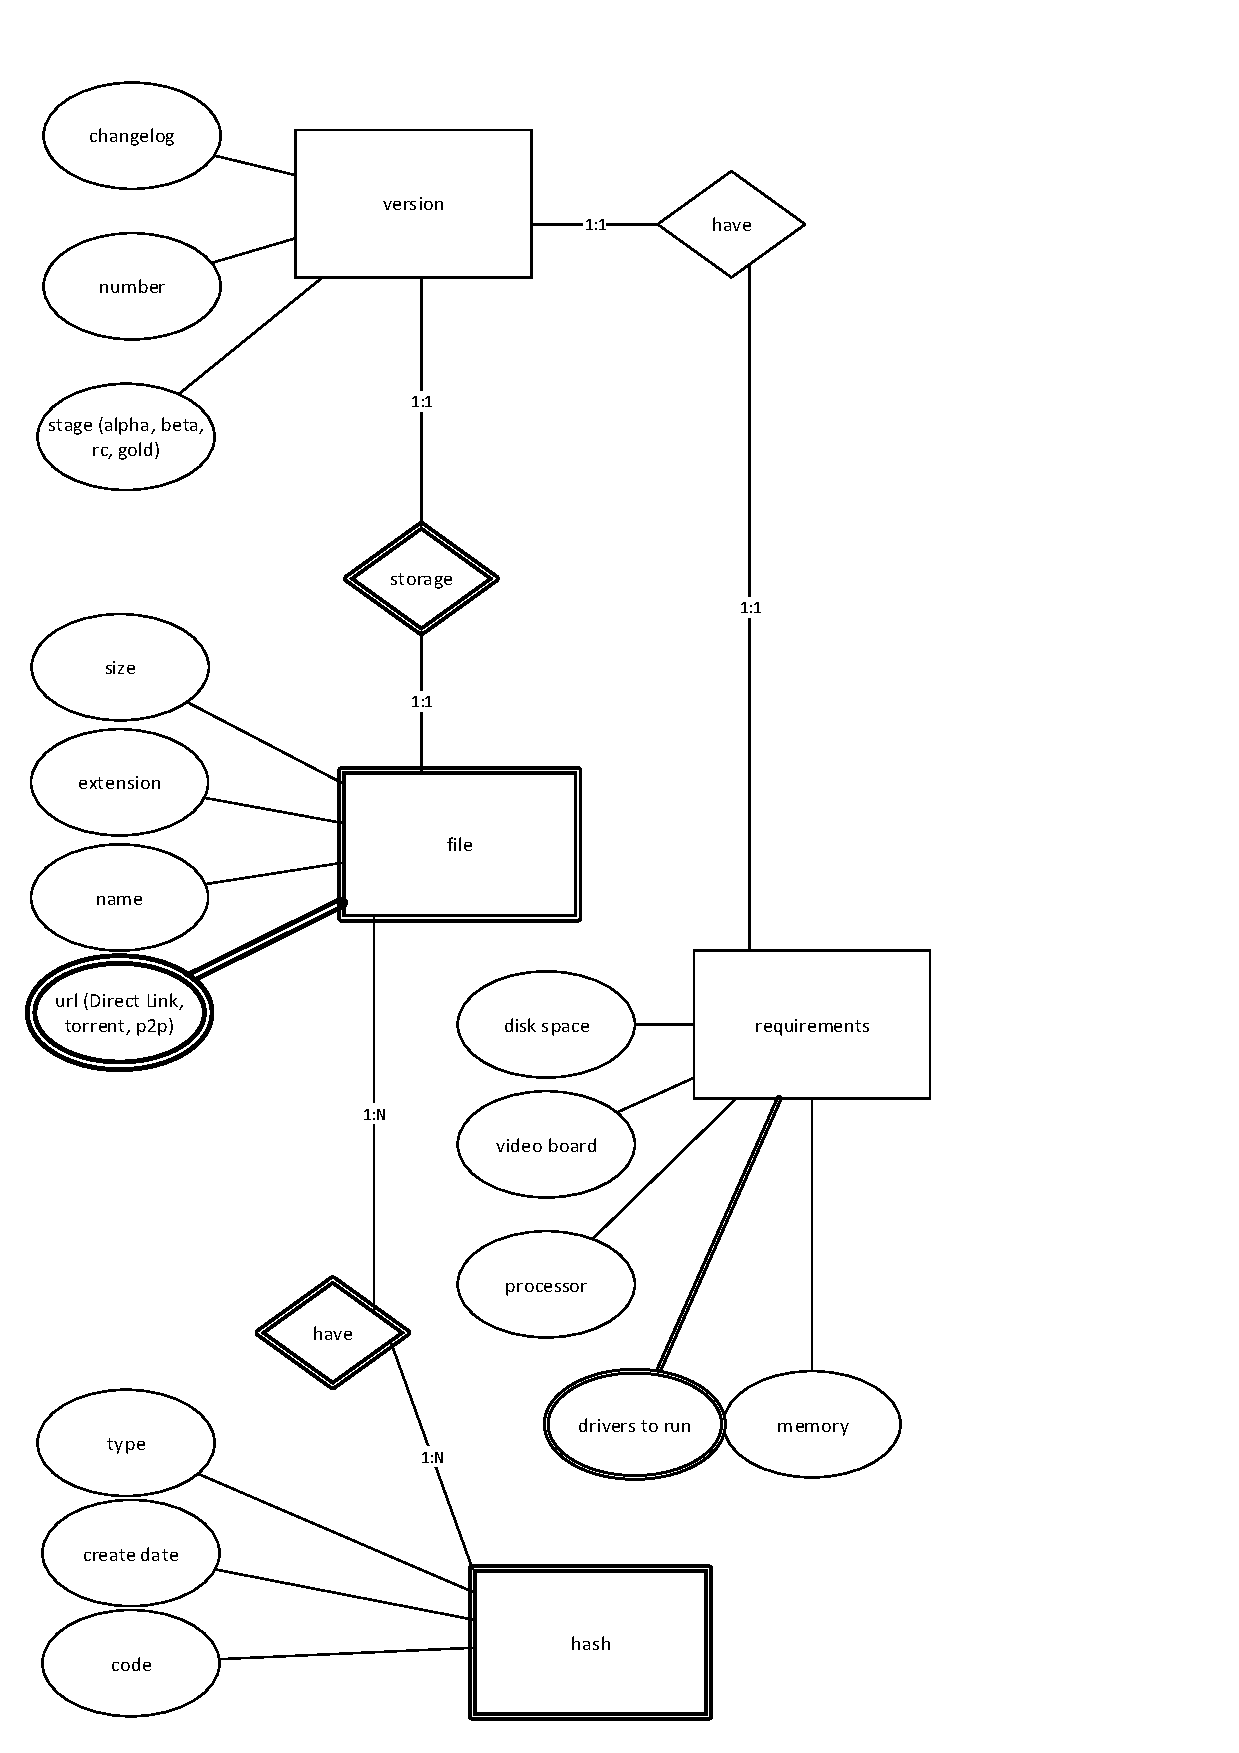
\includegraphics[height=0.95\textheight,width=0.9\textwidth]{MER_-_Version.pdf}
\caption{Entidades responsáveis pelo armazenamento de informações de versões existentes de softwares, animações e livros e seus respectivos arquivos disponibilizados na Web.} \label{hash}
\end{figure}


\begin{figure}[H]
\centering
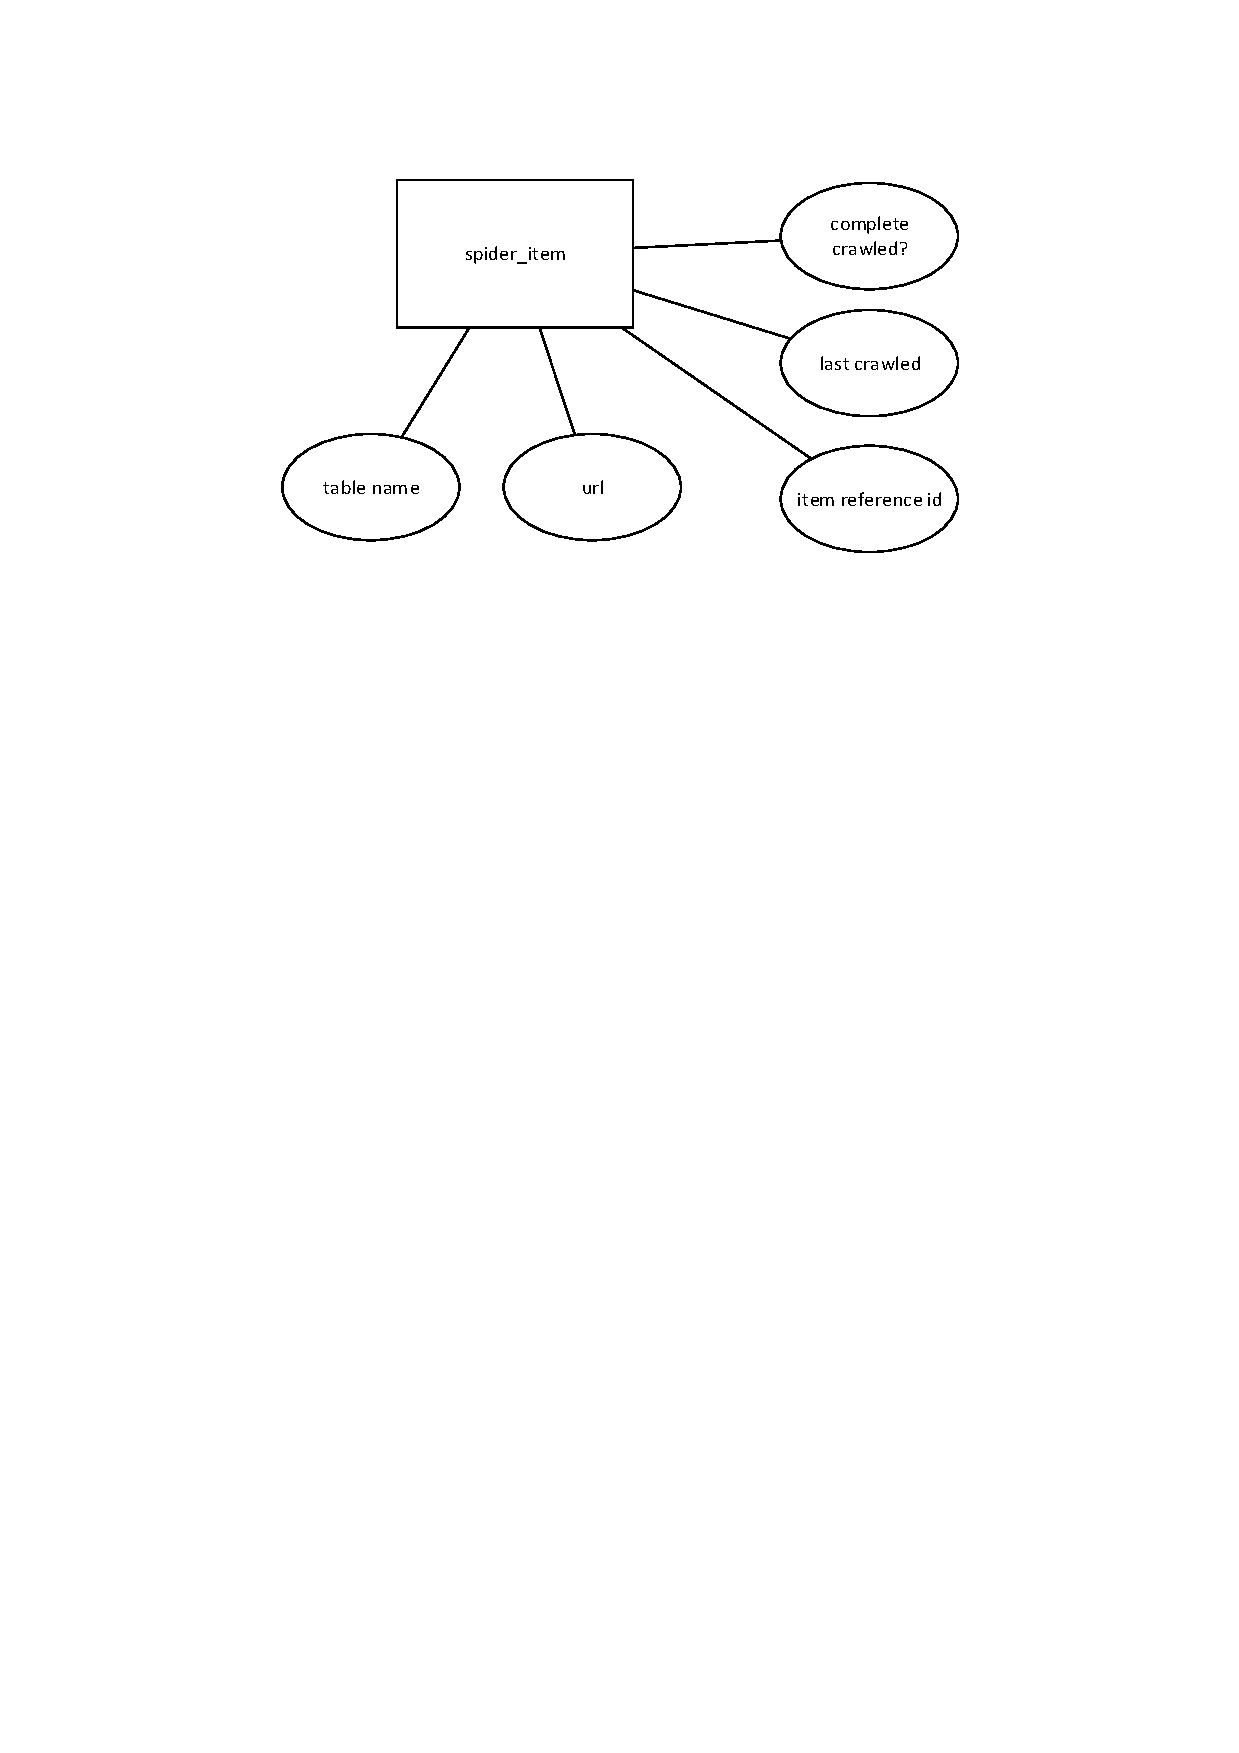
\includegraphics[width=1\textwidth]{MER_-_Spider_item.pdf}
\caption{Entidade responsável pelo armazenamento das URLs que tiveram informações extraídas e salvas no banco de dados. Essa entidade não é utilizada para verificar se uma URL já foi visitada durante uma execução do Crawler, isso é feito no próprio Crawler. Essa entidade serve para garantir que cada URL não salve informações duplicadas em multiplas execuções do Crawler, por isso é salvo a referência do ID e a tabela em que a informação foi salva.} \label{hash}
\end{figure}

\subsubsection{Modelo Relacional}

Após a criação do Modelo Conceitual foram criadas as tabelas e relacionamentos do Modelo Relacional seguindo as três Formas Normais, separando portando atributos multi-valorados, não relacionados a totalidade da chave primaria em tabelas próprias quando necessário.

Também foram criadas chave-primarias não naturais, como índice numérico que serão auto incrementados na inserção de conteúdo, e definido valores padrões para atributos que armazenam Data e Hora.

Para as entidades que possuem mais de um tipo de título ou descrição como \textit{Entity}, \textit{Persona} e \textit{People} que possuem o título principal e título alias foram criadas entidades para armazenamento desses títulos ou descrições com atributo que identifica também o idioma do texto.


\subsubsection{Ferramentas Utilizadas para Modelagem}

\paragraph{Modelo Conceitual\newline}

Para a modelagem do Banco de Dados e criação do Modelo Conceitual foi escolhido o Microsoft Visio que permite a geração de diversos tipos de diagramas, possibilitando a criação de novos itens se necessários para uso nos diagramas. Alguns dos itens como Associação e Atributos Compostos não estão presentes por padrão na modelagem de dados que vem com o Microsoft Visio e tiveram que ser criadas.

\begin{figure}[H]
\centering
\mbox{\subfigure{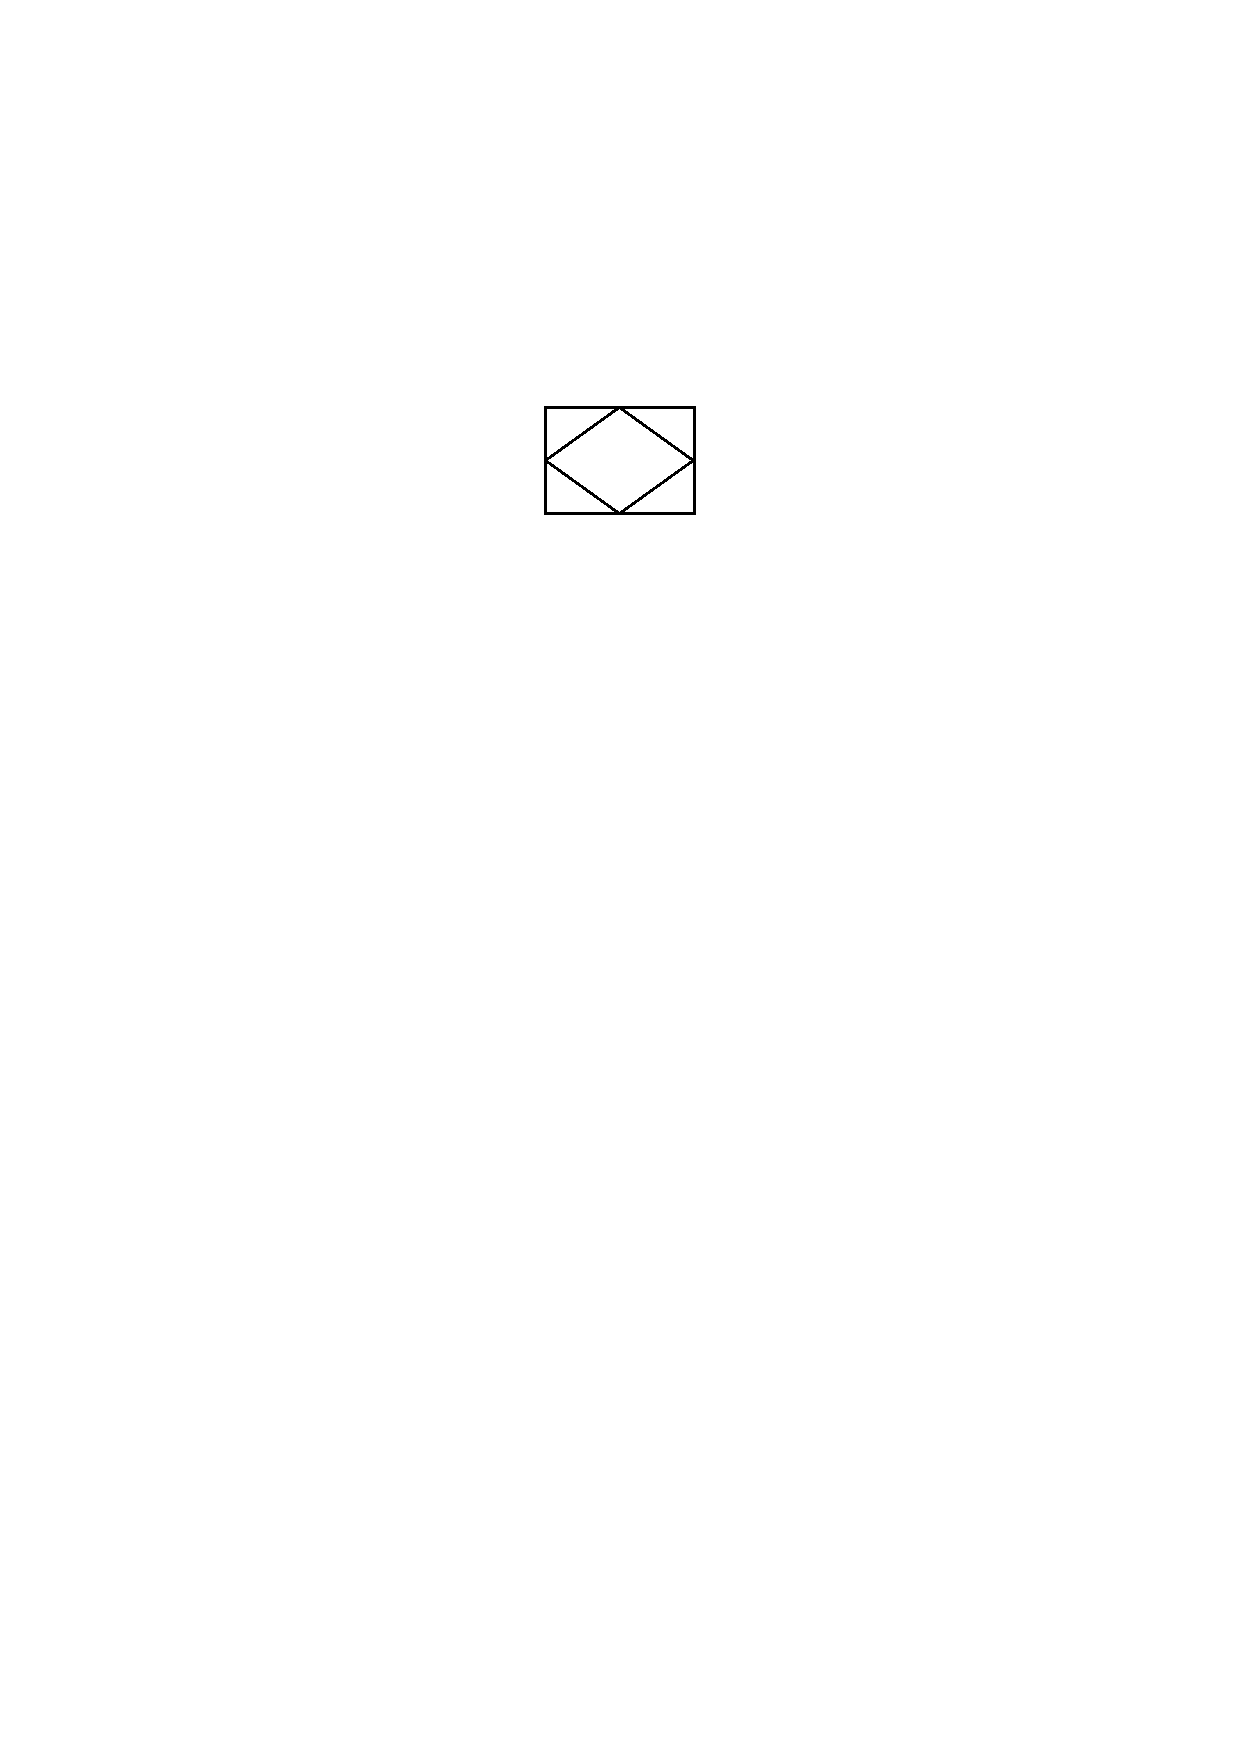
\includegraphics[width=1in]{Generalization.pdf}}\quad
\subfigure{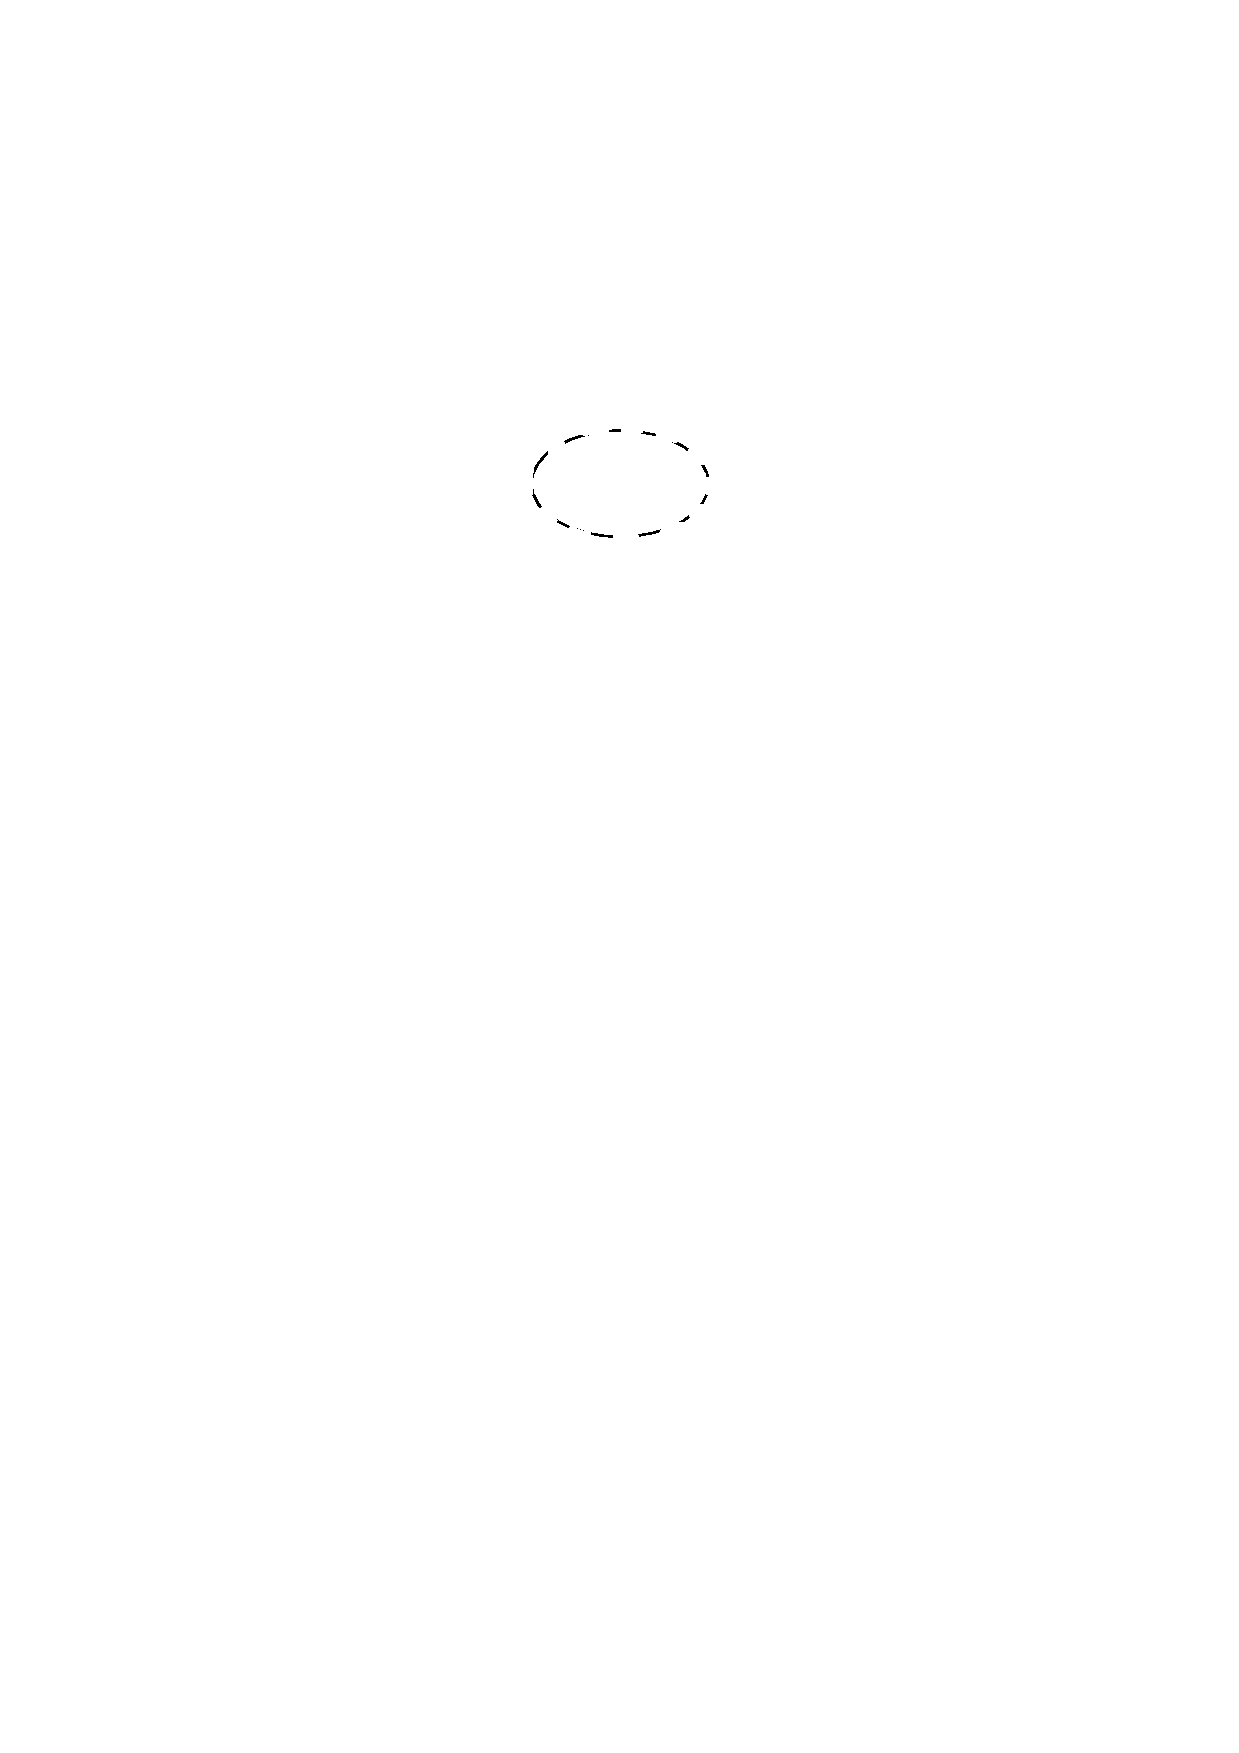
\includegraphics[width=1in]{attribute-derivate.pdf} }\subfigure{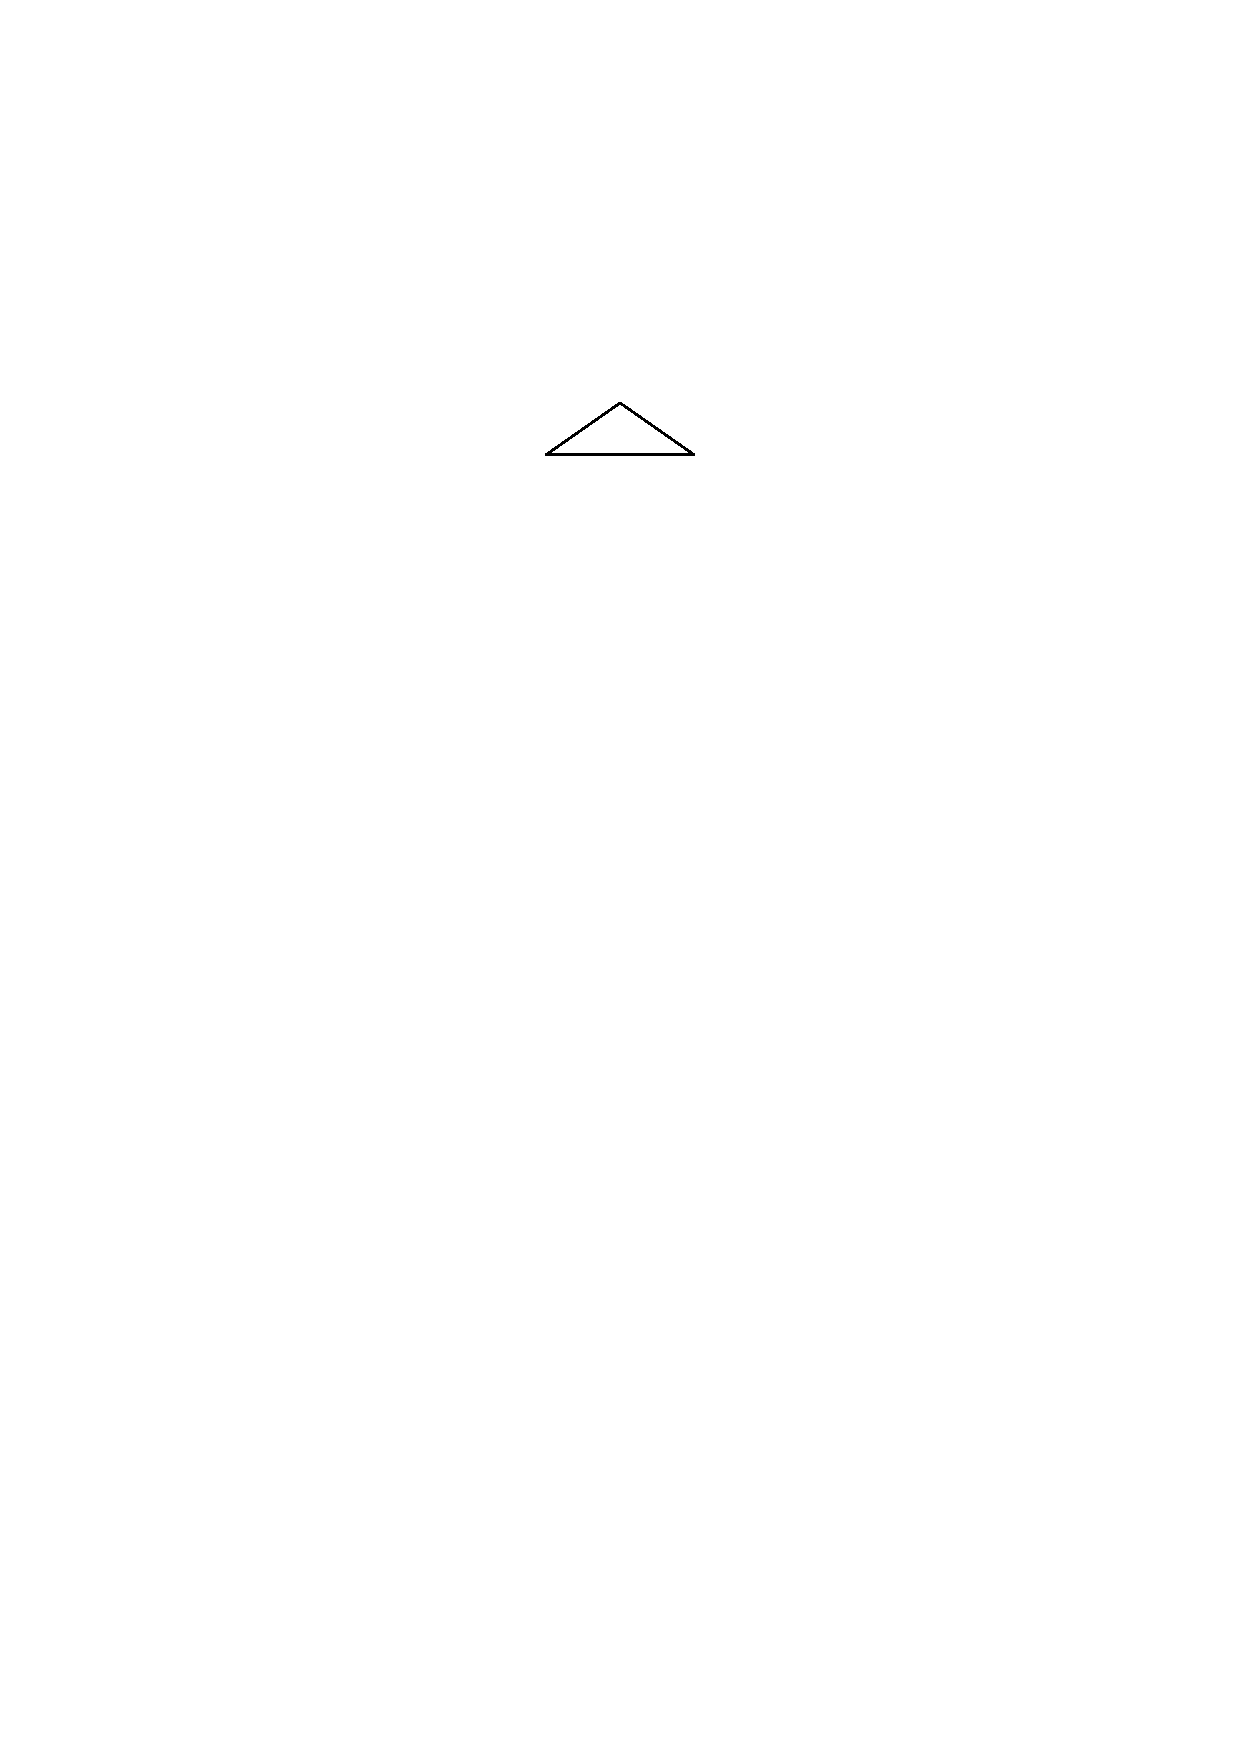
\includegraphics[width=1in]{attribute-generalization.pdf} }}
\caption{Objetos que precisaram ser criados: associação (a), atributo derivado (b) e generalização/especialização (c).}
\label{fig6}
\end{figure}

\paragraph{Modelo Relacional\newline}

Para o Modelo Relacional foi utilizado o DBDesign na sua 4ª versão, que permite a migração do Modelo Relacional para código SQL do MySQL. DBDesign não oferece suporte ao PostgreSQL sendo necessário para criação do Modelo Lógico algumas alterações no arquivo SQL. 

Para um Modelo Relacional extenso o DBDesign porém se mostrou limitado ao não permitir o aumento na área útil em que as entidades poderiam ser adicionadas. Para uma modelagem extensa como a do banco de dados desse projeto essa limitação dificultou a organização pela falta de espaço fazendo com que as entidades ficassem muito próximas umas das outras. 

Além dessa limitação a execução da máquina virtual do JAVA (JVM) para o DB Design apresenta problemas com a hibernação no Sistema Operacional Windows, quando se retorna de uma hibernação, com a JVM ativa, ao tentar salvar ou exportar um arquivo no DBDesign o programa trava sendo necessário reniciar o computador para voltar a utilizar essas opções. Portanto não é recomendo o uso do DB Design para um modelo relacional extenso. 

\paragraph{Modelo Lógico\newline}

Para execução do Modelo Lógico foi utilizado o PostgreSQL 9.3 e o PgAdmin III para o sistema operacional Windows 8. 

Por padrão o usuário inicial no PgAdmin III é o postgres, mas para execução de queries de seleção, inserção e atualização foi criado outro usuário para uso no nosso sistema crawler. 

\subsubsection{Detalhes da Implementação do Modelo Lógico}

Ao exportar o arquivo SQL do DB Design é criado código SQL especificamente para MySQL, para usarmos no PostgreSQL esse código precisou ser alterado.

O código SQL resultante do DB Design possui a criação de índices e chaves-estrangeiras inclusas na criação da própria tabela, apesar de ser compatível com o PostgreSQL resolvemos separ esses código em outros arquivos para uma melhor organização.

No MySQL chave-primárias sequênciais são definidas como valor numérico com propriedade auto\_inclement. Como auto\_inclement não está disponível para o PostgreSQL usamos o equivalente SERIAL.

Código MySQL:

id integer primary key auto\_increment

Equivalente em PostgreSQL:

id serial

Outra própriedade presente no código MySQL que não está disponível em PostgreSQL é o DATETIME, usado para armazenar data e hora. Uma alternativa adotada foi utilizar timestamp, que também armazena data e hora, pórem em microsegundos desde a era Unix (01/01/1970 00:01). Apesar do armazenamento ser diferente se fornecido string concatenada de data e hora no padrão 'AAAA-MM-DD HH:MM:SS' na inserção o PostgreSQL fará a conversão automaticamente para timestamp. 

No PostgreSQL há dois tipos de timestamp: para armazenar com informação de fuso horário e sem informação de fuso horário. Nesse projeto foi escolhido usar armazenamento sem fuso horário (GMT 0) visto que os atributos do banco de dados que usariamos timestamp serviriam para registrar o momento em que os dados foram salvos no banco de dados. Como não foram extraídas informações com data e hora dos websites utilizados não houve necessidade de indicar o fuso horário adotado em cada site para durante a inserção no banco de dados.

Código MySQL:


Alternativa em PostgreSQL:



Um recurso presente em PostgreSQL é a herança entre tabelas, que permitem que tabelas herdem atributos não-chave de outras tabelas. Usamos esse recurso em entidades que possuem especialização, como as entidades \textit{goods} e \textit{edition}. Como herança não é um recurso presente no MySQL durante a criação do Modelo Relacional no DB Design foi utilizado relacionamento de cardinalidade 1:1 entre as tabelas que sofrem especialização/generalização.

O PostgreSQL em sua versão estável mais recente, 9.3, ainda não oferece criação automatizada de relacionamentos e unicidade entre tabelas pais e descendentes quando se indica uma herança na tabela descendente. Atributos chaves-estrageira usados na tabela pai, que também devem estar presentes na tabela descendente, precisam ser inclusos manualmente.

Código para criação de tabela com herança em PostgreSQL:


Uma pesquisa no banco de dados PostgreSQL efetuada em uma tabela pai automaticamente inclui resultados presentes nas tabelas descendentes, para evitar esse comportamento é necessário indicar que se deseja procurar apenas na tabela pai, isso pode ser indicado utilizando ONLY antes do nome da tabela no código SQL de consulta.

Código de consulta em PostgreSQL com ONLY:





\subsection{Crawler}

Um crawler é um programa que visita websites, segue links e extrai informações de páginas especificas. Um crawler deve a partir de uma URL inicial seguir todas as URLs presentes na página a fim de vasculhar o website, critérios podem ser utilizados para indicar quais URLs seguir, como por exemplo o critério de seguir URLs apenas do domínio atual do site, excluindo websites externos de publicidade e redes sociais.

Na execução inicial o Crawler faz o download do código HTML da página da URL inicial e extrai a informação "href" das tags <a> presente na página e as coloca numa lista de processamento usada na analise que determina se a URL deve ser seguida, extraída ou removido da lista. 

Para evitar o problema de loops infinitos quando uma página A possui um link para uma página B e a página B possui link para a página A, deve-se criar uma lista de URLs já visitados para verificação.  
 
Ilustração do Loop aqui. 

Neste projeto foi optado pelo uso de uma biblioteca de crawling que permite o seguimento de URL de páginas e extração de informações sem ter que se preocupar em programar Request e Download de páginas da Web.

A Biblioteca escolhida foi o Scrapy, na versão 0.24.4, desenvolvida em Python, que possibilita a criação da lógica de URLs a serem seguidos usando regras conhecidas como \textit{Rules}. As \textit{Rules} são classes com parametros que definem se as URLs podem ou não ser inseridas na lista de processamento. Esses parametros recebem expressões regulares que serão usadas na analise das URLs. Nas Rules também é definido se a URL deve ter seu conteúdo HTML processado pelo parse ou se deve ter apenas as informações href das tags <a> extraídas.

Como os websites a serem utilizados possuem conteúdo estático sem uso de Ajax o Scrapy atende as necessidades básicas de download e parseamento dos websites. Se for necessário extrair informações dinamicamente geradas por AJAX pode ser utilizado o Scrapy com extensão para Firefox ou outra biblioteca de crawling que permite o download do código-fonte da página como visualizado pelos browser, como a biblioteca Selenium.

Scrapy assim como Python está disponível para Windows e Linux. Nesse projeto foi utilizado a versão compilada para Windows de 64bits.

\subsubsection{Links Duplicados}

Para se evitar o problema de loops durante o crawling, URLs já processadas precisam ser ignoradas durante a extração de URLs de novas páginas.

Adicionar uma URL já processada a uma lista usada para verificação de URLs já visitadas evita esse problema, porém há casos em que duas URLs com mesma quantidade de parametros, mas em ordem diferente, levam a uma mesma página. A fim de evitar re-processar páginas iguais simplesmente pela ordem dos paramêtros estarem diferentes a biblioteca Scrapy não salva as URLs em si, e sim uma representação das URLs mencionadas como "impressão digital" na documentação do Scrapy. 

Para gerar as "impressões digitais" a biblioteca Scrapy reorganiza os paramêtros de uma URL por ordem alfabética e gera a partir da URL resultante o MD5.


Exemplo de URLs que resultam na mesma impressão digital:


https://www.mangaupdates.com/series.html?page=2\&letter=AF

https://www.mangaupdates.com/series.html?letter=AF\&page=2


\subsubsection{Projeto Scrapy}

Scrapy é uma biblioteca com todos os recursos necessários para extrair informações de um website, utilizando \textit{Requests} para download do código-fonte de websites e \textit{Parse} para processamento desse código-fonte. Os Requests e Parses são realizados por meio de classes conhecidas como \textit{Spider}.

Um novo projeto Scrapy pode ser iniciado pela linha de comando e ao ser iniciado será criado uma estrutura pronta de pastas e arquivos padrões com algumas configurações pré-determinadas.
 
"Estrutura de Pastas aqui"

Para a visitação de URLs e extração de dados dos websites a biblioteca Scrapy utiliza as classes \textit{Spider} armazenadas na pasta "spiders", essas classes devem ser herdar de pelo menos um tipo de spider disponível no Scrapy, cada um com sua implementação única.

A classe que escolhemos herdar para criar nossos spiders é a \textit{CrawlSpider} que implementa o método parse, método esse que utiliza as regras definidas para ou seguir uma URL ou efetuar processamento do código-fonte da URL. Quando definimos as regras, em um objeto iterável com nome "rules" na classe, indicamos por meio de expressão regular as páginas que podem ser seguidas e as páginas que devem ter seu conteúdo extraído, parseado e enviado para um método callback. Pode apenas haver um método callback para extração de dados nos spiders que herdam \textit{CrawlSpider}.

Nossa classe spider para ser corretamente executada pela biblioteca Scrapy deve informar a propriedade nome do "spider", dominios permitidos para extração de informação sem o schema "http", as URLs iniciais e as regras de visitação e extração de URL.

Ao criarmos o método callback podemos usá-lo de pelo menos dois modos: 

\begin{enumerate}
\item Usá-lo para armazenar as informações extraídas em objetos conhecidos como \textit{items} para serem depois interpretados por diversos métodos "Pipeline" que verificarão se os "items" estão dentro de uma qualificação lógica adequada para serem salvos em Banco de Dados ou salvos em arquivos Json (Esse é o método recomendado pelo Scrapy)
\item Usá-lo diretamente para salvar as informações sem a necessidade de criação de objetos \textit{items}.
\end{enumerate}

Adotamos esse último método na qual as URLs extraídas e parseadas possuem seus dados normalizados para serem salvos no banco de dados no próprio método callback.
  
%- alguma intenção original foi abandonada? alguma foi adicionada?
 
 
 
\subsubsection{Implementando acesso ao Banco de Dados}

Para acesso ao banco de dados PostgreSQL, em Python, foi utilizado a biblioteca Psycopg2. A biblioteca oferece métodos para conexão com o banco de dados, para execução de código SQL e para controle de transações.

A partir desses métodos básicos criamos uma classe de conexão ao banco de dados, com métodos para inserção e para atualização de dados que manipulem as informações nas tabelas mantendo a integridade lógica dos dados.

\subsubsection{Tratamento de Erros e Transactions}

Muitas das entidades do nosso Modelo Conceitual, na migração para o Modelo Relacional, resultou em diversas tabelas relacionadas. Embora o Banco de Dados seja responsável por manter a integridade quanto aos tipos de dados e existência de chaves-primárias e estrangeiras, ele não se responsabiliza pela integridade lógica dos dados salvos, como por exemplo se a chave-estrangeira associada é a correta ou não para determinado item.

Algumas das páginas processadas pelo \textit{parse} podem ter variações na formatação HTML, que podem originar erros na integridade lógica do Banco de Dados. Assim usando o conceito de \textit{Try Catch} (no Python \textit{Try Exception}), quando ocorre uma falha na inserção de algum conteúdo da página processada pelo \textit{parse} todas as operações executadas com os dados da página são descartadas, usando \textit{Rollback} quando uma Exception ocorre, e a URL da página e informações sobre o erro são inseridas em um arquivo de \textit{Log} para analise posterior.

Somente após realização com sucesso, de todas as operações, é finalmente efetuado \textit{Commit} na transação. Permitindo assim que apenas dados formatados e relacionados corretamente sejam salvos no Banco de Dados.


\subsubsection{Itens Relacionados}

Algumas páginas a terem seu conteúdo extraído possuem lista de itens relacionados, com o nome e URL do item relacionado.

Itens relacionados em que a URL ainda não teve seu conteúdo extraído é salvo com conteúdo em sua maior parte nulo no Banco de Dados, quando a URL desses itens forem extraídas esses itens serão atualizados, mantendo assim o relacionamento entre o conteúdo.


salvos esses itens temporário


Falar que os itens relacionados são salvos no Banco de Dados antes do projeto.
 


e existe, itens sem coleções são al

m é 

código SQL para busca com recursão dos itens relacionados.


identificar a existência 

se já existe uma coleção a 

uma coleção 


, a partir desse conjunto de 

 partir do nome desses itens foi possível criar 

informação  itens possuem 

Ao inserirmos um item ao Banco de Dados que possui conteúdo relacionado 

Ao inserirmos um item ao Banco de Dados, como Mangás, Light Novels verificamos se algum item relacionado

As coleções foram criadas durante a execução do Crawler, 

 no próprio código, outras só poderiam ser analisadas após o termino 

 a que cada item pera partir dos Websites.


Para tal precisávamos criar as coleções e relacionar os diversos tipos de itens (como mangás, light novels, etc) a uma coleção.



em uma coleçção


e englobar diversos itens






\subsubsection{Definindo Coleções}

Para alcançarmos o objetivo de fazer uma visualização de dados com extração de informações relacionadas a coleções, precisávamos identificar e criar as coleções a partir do conteúdo salvo no Banco de Dados.

Durante a extração de dados pelo Crawler algumas páginas forneciam também o nome e URLs para itens relacionados. Com os itens relacionados foi possível verificar se já existe uma coleção associada a algum dos itens ou criar uma nova coleção se inexistente.

Para identificar se existe uma coleção já salva no Banco de Dados foi executado uma busca recursiva a fim de retornar todos os itens relacionados entre si, utilizando o recurso WITH RECURSIVE do PostgreSQL.

Se existe alguma coleção associada a um item essa coleção é utilizada para associar a itens ainda sem coleção. Se não existir alguma coleção salva no Banco de Dados, casos em nenhuma coleção foi criada ainda na execução do Crawler a coleção é criada.

(Separação de títulos)
Para a criação da coleção é utilizado a parte dos títulos anteriores a caracteres usados para divisão de subtítulos como hifen " - " e parenteses "()", o texto após extraido é formatado e utilizado para criação da coleção. 
Em casos com itens relacionados com títulos diferentes o título mais comum será usado.  


Exemplo:
		Fairy Tail
		Fairy Tail Freezing

		

Com esse método há possibilidade de associar em coleções itens com nomes semelhantes que pertencem a coleções distintas. Para corrigir casos assim é necessário uma verificação manual da associação de Coleções.



\subsection{Visualização de Dados}

Para visualização de dados extraímos do Banco de Dados textos e representamos a variação na quantidade entre os textos, exibindo-as como uma nuvem de bolhas ou uma nuvem de palavras. 
Usamos a estrutura de dados Tabela de Área Somada[] para identificação de espaços ocupados e realizamos uma distribuição aleatória na imagem de nossos objetos: as bolhas ou as palavras.
Para esse fim utilizamos a biblioteca Numpy para manipulação de vetores multidimensionais, gerando assim a Tabela de Área Somada, e a biblioteca PIL para desenhar palavras, desenhar formas e salvar a imagem resultante.

A Figura número-aqui ilustra a seqüência adotada para identificação do espaço e o tamanho da bolha ou da palavra a ser utilizada. Essas etapas serão melhor explicadas nos próximos tópicos.   

\subsection{Preparando a Cena}

Utilizando a biblioteca de processamento de imagem preparamos um fundo com tamanho determinado que usaremos para posicionar nossos objetos. 
Qualquer seguimento da Tabela de Área Somada com valor diferente de zero é considerado ocupado, assim podemos criar uma imagem com fundo totalmente preto, utilizando toda a área disponível, ou podemos criar uma área limitada com ilustrações ou textos resultando em uma máscara para nossa visualização.
A cor preta é representada pelo valor 0 e ao converter a imagem preparada em um vetor multidimensional com Numpy obtemos a Tabela de Área Somada inicial.


Imagem exemplo de Máscara. => Representação Vetorial


\subsection{Definindo o Tamanho dos Objetos}

Ao obtermos nossos objetos, palavras e círculos, do Banco de Dados também selecionamos informação numérica que representam um ranking entre os objetos, como quantidade de itens da Coleção, valor em reais para adquirir cada item da coleção, volume que a coleção ocupa entre outras informações numéricas.

Alguns dos valores usados para Rankeamento:


Para definir o tamanho dos objetos usamos a razão do valor do Rankeamento pelo logaritmo natural desse valor nas formulas:

Dividimos por 10 para que ranking acima de 1000 não gerem tamanhos demasiadamente grandes. 

{Calculo aqui}

Para evitar divisão por zero é somado o valor 10 ao número do rankeamento antes do cálculo do Logaritmo Natural.

 


Nossos objetos, palavras e círculos, são representam informações extraídas do Banco de Dados com duas informaçõesCada objeto possui 


Para cada objeto h
Cada objeto possui



\subsection{Determinando a posição dos Objetos}

Na cena os objetos não podem sobrepor uns aos outros, para verificarmos os espaços disponíveis para inserção do objeto na cena sem sobrepor outros objetos na cena foi utilizado a Tabela de Área Somada, também conhecida em Estatística como Tabela de Distribuição Acumulada e como Imagem Integral em Visão Computacional.

Para uso da Tabela de Área Somada é utilizado imagens na escala cinza, assim podemos trabalhar apenas um um valor variante para cada pixel da imagem. 

Tabela de área somada


$I(x,y) = \sum_{\begin{smallmatrix} x' \le x \\ y' \le y\end{smallmatrix}} i(x',y')$

Para verificar se um espaço está disponível na cena para nossos objetos precisávamos verificar se já não existe outro objeto já posicionado no local. 

Conseguimos verificar se o espaço está ocupado calculando a área com os valores da Tabela de Área Somada a tempo constante utilizando a fórmula de Área da Imagem Integral. Como utilizamos uma cena em escala cinza, qualquer espaço ocupado resultará em uma soma com valor acima de zero.  

$\sum_{\begin{smallmatrix} x0 < x \le x1 \\ y0 < y \le y1 \end{smallmatrix}} i(x,y) = I(D) + I(A) - I(B) - I(C).$

Para obtermos uma melhor distribuição dos objetos na cena verificamos todos os espaços disponíveis, obtendo a Área da Imagem Integral em todos os pixels da cena. Os valores de x e y livres são portanto armazenados em um vetor e uma única posição é escolhida aleatoriamente como local do nosso objeto. 


\subsubsection{Gerando a Imagem Final}


\subsubsection{Exportando para HTML}

Com a determinação do posicionamento dos objetos na cena, tamanhos e fontes de texto utilizadas além de gerar uma imagem final também podemos exportar nossa nuvem para HTML utilizando CSS para desenhar e posicionar nossos objetos dentro de uma tag <div>.

A posição dos objetos é relativa a tag <div>, as mesmas coordenadas [x, y] utilizadas no posicionamento em nossa imagem podem ser aplicadas na tag.

Geramos um documento HTML com nosso CSS adicionado na tag <head>, para melhor manipulação de nossos objetos. dentro da tag <div> principal, os colocamos em tags <div> separadas possuindo classes para representarmos os tamanhos, formas e posições.

A conversão para HTML foi simples, para as formas e textos, ao invés de utilizar os métodos fornecidos pela biblioteca de processamento de imagem criamos métodos que retornem a representação em CSS das formas utilizadas (círculos) e a representação dos textos com posicionamento definido usando os mesmos parâmetros disponíveis. 
Formatamos portanto o documento HTML com o CSS e as tags <div> de nossos objetos.


\section{Resultados}

Com o uso de crawling foi possível obter uma quantidade considerável de dados. Um resultado mais detalhado pode ser visto a seguir: 

Manga-Updates - Com o crawling do site http://mangaupdates.com foi possível obter 103774 itens, classificados como Mangás, Light Novels e livros; 34721 pessoas, que atuam como ilustradores ou escritores; e 1181 editoras.

My Figure Collection - Com o crawling do site http://myfigurecollection.net foi possível obter 205041 produtos, incluindo Figuras e 3440 empresas envolvidas na produção desses produtos.

Anime Characters Database - Com o crawling do site http://animecharactersdatabase.com/ foi possível obter informações de 70304 personagens e 4840 dubladores.

Com os resultados obtidos com o crawling foi possível criar 109274 coleções e associá-las aos itens e aos produtos. Também foi possível relacionar produtos com personagens.

Para obter esses resultados foi necessário a execução do crawler por três dias consecutivos, levando um dia para download e extração das informações de cada site.  

Com as informações armazenadas no Banco de Dados foi possível criar várias visualizações seguindo os dois modelos de visualizações desenvolvidos nesse projeto.




Figura


Figura


Figura


Figura


Figura



Para ambos os modelos o tempo de processamento é similar, e dependendo da quantidade de objetos (palavras ou círculos), a serem utilizados, podem ser processados em alguns minutos, em casos com 10 objetos, ou em 12 horas, em casos com 10.000 objetos. A maior parte do tempo é consumida pela busca por espaço disponível. 

Quando um espaço não for encontrado o objeto sofre redução no seu tamanho e novamente é procurado por um espaço disponível. A redução é realizada a cada 1 pixel. 




Resultados.
Quais foram os dados considerados? Qual é o volume desses dados? Quanto tempo foi
necessário para obtê-los e armazená-los? Quais visualizações foram consideradas interessantes e quais não
foram? Quanto tempo foi necessário para gerar essas visualizações? Alguma delas foi surpreendente?


\bibliographystyle{plain}
\begin{thebibliography}{2}

\end{thebibliography}
\end{document}